\documentclass[10pt,twoside,titlepage]{seamless}
\usepackage{amsmath}
\usepackage{amssymb}
\usepackage{color}
\usepackage{times}
%\usepackage{fullpage}
\usepackage{graphicx}
\usepackage{listings}
\usepackage{longtable}
\usepackage[nottoc]{tocbibind}
\usepackage{multirow}
\usepackage{wrapfig,booktabs}
\usepackage{subcaption}
%\usepackage{cleveref}
%%
% These are special environments for adding extra information about
% code snippets which can be later extracted and used to generate test
% codes for automated testing.
%
% During LaTeX compilation, the environments defined in this file throw
% away all text within the scope of the environment, with the
% exception of 'chapelprintoutput' which prints the output (and is
% also extracted for testing purposes).
%
% Usage:
%
% - chapelexample (REQUIRED) {f.chpl}
%   This marks the start of a test.  This environment requires a
%   single argument that is the name of the Chapel test program.  This
%   filename will appear in the spec.
%
% - chapelpre
%   Any Chapel code in this scope is put *before* the code in the
%   chapel|chapelcode scope.
%
% - chapelcode|chapel
%   This is the part of the code that is in the spec.
%
% - chapelnoprint
%   This is the part of the code that goes in the test with chapelcode
%   and chapel, but does not appear in the spec.
%   
% - chapelpost
%   Any Chapel code in this scope is put *after* the code in the
%   chapel|chapelcode scope.
%
% - chapelfuture
% - chapelcompopts
% - chapelexecopts
%   The lines in these scopes are put directly into the appropriate file.
%
% - chapeloutput|chapelprintoutput (REQUIRED)
%   These environment provide the test output (.good files).  There can be
%   multiple such environments, and the filename is specified by a LaTeX
%   style comment preceeding the contents of the output.  The
%   'chapelprintoutput' scope is also outputted in the spec itself and
%   thus may contain LaTeX formatting (see GENERAL CAVEATS below)
%   
% - chapelwideoutput
%   Provides the test output for no-local tests, if that differs from the
%   normal test output.  The content of this environment is dumped into a
%   <test>.no-local.good file, along with a copy of the content of 
%   chplprintoutput.
%

%
% GENERAL CAVEATS:
%
% - Because the chapelprintoutput environment must used LaTeX
%   formatting, the script that extracts the tests must removed any
%   LaTeX specific formatting.
%
% - Using a backslash or other special LaTeX characters may also be
%   needed (e.g., \_ or \#) in the other environments for LaTex
%   parsing purposes.  Such characters are considered fragile and may
%   lead to unexpected results.
%

%
% Gobble up the text in this new box.  The text in each environment is
% dropped on the floor during LaTeX compilation.
%
\newsavebox{\teststuff}

%
% Any additional lines needed for the code snippet to run/compile
% (before and after the chapel code segment)
%
\newenvironment{chapelpre} {\begin{lrbox}{\teststuff}
\begin{minipage}{6in}}
{\end{minipage}\end{lrbox}}

\newenvironment{chapelnoprint} {\begin{lrbox}{\teststuff}
\begin{minipage}{6in}}
{\end{minipage}\end{lrbox}}

\newenvironment{chapelpost} {\begin{lrbox}{\teststuff}
\begin{minipage}{6in}}
{\end{minipage}\end{lrbox}}


%
% .future file
%
\newenvironment{chapelfuture} {\begin{lrbox}{\teststuff}
\begin{minipage}{6in}}
{\end{minipage}\end{lrbox}}

%
% .compopts file
%
\newenvironment{chapelcompopts} {\begin{lrbox}{\teststuff}
\begin{minipage}{6in}}
{\end{minipage}\end{lrbox}}

%
% .execopts file
%
\newenvironment{chapelexecopts} {\begin{lrbox}{\teststuff}
\begin{minipage}{6in}}
{\end{minipage}\end{lrbox}}


%
% .good file
% To get more than one file, use a LaTeX style comment to name the
% .good file
%
\newenvironment{chapeloutput} {\begin{lrbox}{\teststuff}
\begin{minipage}{6in}}
{\end{minipage}\end{lrbox}}

%
% .no-local.good file
% (The naming feature mentioned above does not yet work, so this
% environment is a Q&D way to get a .no-local.good file.)
%
\newenvironment{chapelwideoutput} {\begin{lrbox}{\teststuff}
\begin{minipage}{6in}}
{\end{minipage}\end{lrbox}}

%
% .prediff file
%
\newenvironment{chapelprediff} {\begin{lrbox}{\teststuff}
\begin{minipage}{6in}}
{\end{minipage}\end{lrbox}}

%
% .good file that is printed in the text of the Spec
% To get more than one file, use a LaTeX style comment to name the
% .good file
%
%\lstnewenvironment{chapelprintoutput} 
% (See chapel_listing.tex for the implementation.)

\usepackage{seamless}
\lstdefinelanguage{chapel}
  {
    morekeywords={
      align, atomic,
      begin, bool, break, by,
      class, cobegin, coforall, complex, config, const, continue,
      delete, dmapped, do, domain,
      else, enum, extern, export,
      false, for, forall,
      if, imag, in, index, inline, inout, int, iter,
      label, lambda, let, local, locale,
      module,
      new, nil, noinit,
      on, opaque, otherwise, out,
      param, proc,
      range, real, record, reduce, ref, return,
      scan, select, serial, single, sparse, string, subdomain, sync,
      then, true, type,
      uint, union, use,
      var,
      when, where, while, with,
      yield,
      zip
    },
    sensitive=false,
    mathescape=true,
    morecomment=[l]{//},
    morecomment=[s]{/*}{*/},
    morestring=[b]",
}

\lstset{
    basicstyle=\footnotesize\ttfamily,
    keywordstyle=\bfseries,
    commentstyle=\em,
    showstringspaces=false,
    flexiblecolumns=false,
    numbers=left,
    numbersep=5pt,
    numberstyle=\tiny,
    numberblanklines=false,
    stepnumber=0,
    escapeinside={(*}{*)},
    language=chapel,
  }

%\newcommand{\chpl}[1]{\lstinline[language=chapel,basicstyle=\ttfamily,keywordstyle=\bfseries]!#1!}
\newcommand{\chpl}[1]{\lstinline[language=chapel,basicstyle=\small\ttfamily,keywordstyle=]!#1!}
\newcommand{\varname}[1]{\emph{#1}}
\newcommand{\typename}[1]{\emph{#1}}
\newcommand{\fnname}[1]{\chpl{#1}}

\lstnewenvironment{chapel}{\lstset{language=chapel,xleftmargin=2pc,stepnumber=0}}{}
\lstnewenvironment{invisible}{\lstset{language=chapel,xleftmargin=2pc,stepnumber=0,keywordstyle=\bfseries\color{white},basicstyle=\small\ttfamily\color{white}}}{}
\lstnewenvironment{chapel0}{\lstset{language=chapel,stepnumber=0}}{}

\lstnewenvironment{numberedchapel}{\lstset{language=chapel,xleftmargin=15pt,stepnumber=1}}{}

\lstnewenvironment{chapelcode}{\lstset{language=chapel,stepnumber=1}}{}

% Uses the same listing style as the {chapel} environment, but keyword
% formatting is turned off.  The argument is ignored in LaTeX
% but used to name the .good file during test extraction.
% The argument must be supplied but may be empty.
% If empty it defaults to null, which signals the test extractor to 
% autogenerate the .good file name as ``<test_name>.good''.
\lstnewenvironment{chapelprintoutput}[1]
  {\lstset{language=chapel,xleftmargin=2pc,stepnumber=0,keywordstyle=}}{}

\lstnewenvironment{commandline}{\lstset{keywordstyle=,xleftmargin=2pc}}{}

\lstnewenvironment{protohead}{\lstset{language=chapel,xleftmargin=0pc,belowskip=-10pt,stepnumber=0}}{}

\newenvironment{protobody}{\begin{description}\item[\quad\quad] }{\end{description}}


%% High section numbers require different number widths
\usepackage[titles]{tocloft}
\setlength{\cftchapnumwidth}{1.3em} % Wide enough for a chapter number.
\setlength{\cftsecnumwidth}{3.2em}  % Same as cftsubsecnumwidth:
\setlength{\cftsubsecnumwidth}{3.2em} % Wide enough for three digits and two dots.
%\setlength{\cftsubsubsecnumwidth}{5.4em}
\setlength{\cftsecindent}{1.3em}    % cftchapnumwidth
\setlength{\cftsubsecindent}{1.3em} % cftchapnumwidth
\setlength{\cftsubsubsecindent}{4.5em} % cftchapnumwidth + cftsecnumwidth

%\usepackage{ifpdf}
%\ifpdf
%\usepackage[pdftex,
            %bookmarks,
            %plainpages=false,
            %breaklinks,
            %pdftitle={Test-Driven Development with seamless},
            %pdfauthor={Paul Adamson},
            %pdfsubject={seamless package, literate programming, test-driven development}
           %]{hyperref}
%\else
%\usepackage[ps2pdf]{hyperref}
%\fi

% some custom latex convenience commands
\usepackage{xspace}
\newcommand*{\eg}{\emph{e.g.}\@\xspace}
\newcommand*{\ie}{\emph{i.e.}\@\xspace}

\makeatletter
\newcommand*{\etc}{%
  \@ifnextchar{.}%
  {etc}%
  {etc.\@\xspace}%
}
\makeatother

\newcommand{\rsec}[1]
           {\S\ref{#1}}

% courtesy: http://www.iam.ubc.ca/~newbury/tex/page-set-up.html
\newcommand{\sekshun}[1]
           {
             \chapter{#1}
             \markboth{Test-Driven Development with \texttt{seamless}}{#1}
           }

\oddsidemargin 0.0in
\evensidemargin 0.5in
\textwidth 6in
\headheight 0.2in
\topmargin 0in
\headsep 0.3in
\textheight 8.5in

\makeindex
\title{Test-Driven Development with \texttt{seamless}}

\author{Paul Adamson\\
\\
}

\date{January 1, 2015}

\setcounter{tocdepth}{3}

\begin{document}

\pagestyle{empty}
%\pagenumbering{alph}

\ifpdf
\pdfbookmark[1]{Title}{titlepage}
\fi
\maketitle

\null\vfill
\noindent
\begin{center}
\copyright Paul Adamson
\end{center}

\cleardoublepage
\include{tm}
\cleardoublepage

\pagestyle{myheadings}
\markboth{Test-Driven Development with \texttt{seamless}}{Test-Driven Development with \texttt{seamless}}
%\pagenumbering{roman}

\ifpdf
\pdfbookmark[1]{Table of Contents}{tablecontents}
\fi
\tableofcontents

\cleardoublepage

\pagestyle{myheadings}
%\pagenumbering{arabic}

\setlength{\parindent}{0in}
\setlength{\parskip}{4mm plus2mm minus1mm}

%\part{Introduction}
\sekshun{Tutorial Introduction}
\label{Tutorial_Introduction}

\begin{TODO}
  Introduction.
\end{TODO}

Before we dive into developing requirements and hacking away at code, a brief description of 
the \lstinline{seamless} approach to software development, a literate programming approach to 
test-driven development, is in order.  (Well, as you will see later, the \lstinline{seamless} approach
is probably better described as a ``quasi-literate programming'' approach, but I will explain
in due course.)

\section{Test-Driven Development}
Test-driven development, or TDD, is the notion that developers will improve both the design and
accuracy of their code by \textit{writing the test} for a particular feature \textit{before writing the 
code} that implements the feature according to the specification. In other words, the TDD process 
begins with writing an automated test for code that does not yet 
exist. After a test is written for a particular feature defined in the specification, the 
programmer then writes the implementing code to get the test to pass. This process is repeated until
all features in the specification are implemented. 

The idea is that by writing tests before code, rather than after, the tests will help guide
the design in small, incremental steps. Over time, this creates a well-factored and robust
codebase that is easier to modify.

\begin{TODO}
Consider adding a story about TDD.
\end{TODO}

\subsection{The Classic TDD Process}\label{tdd-classic}

\begin{TODO} The following process is almost ver batim from Rails 4 Test Prescriptions. Need to 
cite the work and tailor to technical computing/Chapel code development.
\end{TODO}

The classic TDD process goes something like this:
\begin{enumerate}
\item Create a test. The test should be short and test for one thing in your code. The test
should run automatically.
\item Make sure the test fails. Verifying the test failure before you write code helps ensure
that the test really does what you expect.
\item Write the simplest code that could possibly make the test pass. Don't worry about good
code yet. Don't look ahead. Sometimes, write just enough code to clear the current error.
\item After the test passes, refactor to improve the code. Clean up duplication. Optimize.
Create new abstractions. Refactoring is a key part of design, so don't skip this. 
\item Run the tests again to make sure you haven't changed any behavior.
\end{enumerate}

Repeat the above cycle until your code is complete. This will, in theory, ensure that your code is
always as simple as possible and completely covered by tests. 

\subsection{TDD Aids Design}

\begin{TODO}
Describe in more detail how TDD aids design. Draw from Rails Test Prescriptions, pg 5+.
\end{TODO}

\subsection{Tests as Code Documentation}
A case can be made in some domains (e.g. web development) that automated test suites 
provide an alternate means of documenting code--that
the tests are, in essence, a detailed specification of the code's behavior. This is somewhat true in
technical computing, but full documentation of scientific and engineering software requires 
more than just brief comments and example output. Surely, documentation for a function that computes 
the electron-electron repulsion integral in a quantum chemistry code must have some description
of the type of electronic wavefunction for which the code is valid!

\section{Literate Programming}
Enter stage right...literate programming. 

A typical computer program consists of a text file 
containing program code. Strewn throughout will likely be scant plain text descriptions separated out by 
``comment delimeters'' that document various aspects of the code.
Since the actual code itself is presented in a such a way that supports the syntax, ordering, and structure 
that the programming language (and hence compiler) requires, the code comments will
be relatively disorganized and disjointed if you are reading them for documentation purposes. 
The way a code suite is organized in source is generally much different than the way thorough documentation is 
developed. The plain text nature of the comments also greatly limits their information value.

In literate programming the emphasis is reversed. Instead of writing \textit{a lot of} code that contains 
\textit{some} plain text documentation, 
the literate programmer writes \textit{thorough, well-organized, and content-rich} documentation that contains 
\textit{modular and efficient} code. 
The result is that the commentary is no longer hidden within a program surrounded by 
comment delimiters; instead, it is made the main focus. 
The ``program'' becomes primarily a document directed at humans, with the 
code interspersed within the documentation, separted out by ``code delimiters'' so that it can be extracted 
out and processed into source code by literate programming tools. The nature of literate programming is 
summarized pretty well in a quote from the online documentation for the FunnelWeb literate programming
preprocessor:

\begin{quote}
``The effect of this simple shift of emphasis can be so profound as to change one's whole approach to
programming. Under the literate programming paradigm, the central activity of programming becomes that of 
conveying meaning to other intelligent beings rather than merely convincing the computer to behave in a 
particular way. It is the difference between performing and exposing a magic trick.'' 
\begin{flushright}
-FunnelWeb Tutorial Manual\cite{funnelweb-what-is-literate-programming}
\end{flushright}
\end{quote}

\label{literate-program-requirements}
The following list of requirements can be used to define a ``literate program:''\cite{childs}
\begin{enumerate}
\item The high-level language code and the associated documentation come from the same 
set of source files.
\item The documentation and high-level language code for a given aspect of the program should be 
adjacent to each other when presented to the reader.
\item The literate program should be subdivided in a logical way.
\item The program should be presented in an order that is logical from the standpoint of documentation
rather than to conform to syntactic constraints of the underlying programming language(s).
\item The documentation should include notes on open issues and future areas for development.
\item Most importantly, the documentation should include a description of the problem and its solution. 
This should include all aids such as mathematics and graphics that enhance communication of the problem 
statement and the understanding of its challenge.
\item Cross references, indices, and different fonts for text, high-level language keywords, 
variable names, and literals should be reasonably automatic and obvious in the source and the documentation.
\item The program is written in small chunks that include the documentation, definitions, and code.
\end{enumerate}

The documentation portion may be any text that aids the understanding of the problem solved by the code 
(\eg description of the algorithm that is implemented).  The documentation is often significantly 
longer than the code itself. Ideally, the problem is described in a way that is agnostic of the language
in which the code is written.  For example, documentation for code that integrates a function $f(x)$ would
have discussion of discontinuities, various integration methods available (\eg trapezoidal, Simpson), 
domain of integration, \etc. 
In addition to basic shortfalls in documentation and testing in scientific codes, a recent 
study highlighted the widespread lack of basic context in available documentation.\cite{petre}
Literate programming solves this problem, ensuring that context is created while the program
is written.

\section{Literate Programming Approach to Test-Driven Development}
Test-driven development and literate programming are certainly compatible.  In fact, they are 
complementary and their combined use is a rare actual example of ``the whole is greater
than the sum of its parts,'' especially in the context of developing scientific code.  
In one document, we can clearly outline the problem to be solved, develop a test for the 
code that we want, and document the code that solves the problem. As this is done in an incremental
manner, the scientist develops the code that solves the right problem in an efficient and robust manner.
As will be seen below, the proccess also supports several fundamental aspects of good software
engineering.

\subsection{A Better TDD Process}\label{tdd-better}

\begin{TODO}
Describe why you must begin with good requirements.
\end{TODO}

A better TDD process begins first with a ``good'' requirement specification.
Failing to write a specification is the single biggest unnecessary risk a developer
can take in a software project, resulting in greatly diminished productivity. 
For any non-trivial project (more than a few days of coding for one programmer), 
the lack of a thorough specification will always result in more time and lower quality code.
Even for trivial examples, a short, informal specification will at least help to ensure
accuracy of the resulting code.

The specification is the high-level design of the program. 
Most importantly, it clearly defines the problem that the program will solve. 
Of almost equal importance is the specification of the
basic algorithms and outputs of the code. During development of the requirement specification,
the developer should evaluate available algorithms and consider how data produced from the 
program will be used.
Even if a spec is written solely for the benefit of a lone developer, the act of 
writing the specification---describing how the program works in 
minute detail---will force design of the program.

Once a specification is in hand, an improved TDD process (section \ref{tdd-classic}) can be 
undertaken in context of literate programming:
\begin{enumerate}
\item Document the problem and its solution.
  \begin{enumerate}
  \item Describe a small part of the problem to be solved. The description should include    
all aids such as mathematics and graphics that enhance communication of the problem 
statement and the understanding of its challenge. 
  \item Solve the problem, again using all aids at your disposal (\eg math, graphics).
  \item Include appropriate references to higher level requirement specifications.
  \end{enumerate}
\item Create a test. 
\begin{enumerate}
  \item The test should be as short as possible and test for one solution in your overall
  problem.\footnote{Note here that ``one thing in your code'' is replaced with ``one
  solution in your overall problem.'' This change emphasizes the literate programming emphasis
  on documenting the problem and solution before writing code. Writing the test is another
  form of documenting the solution.}
  \item The test should run automatically.
  \item Make sure the test fails. 
\end{enumerate}
\item Create the code.
  \begin{enumerate}
  \item Write the simplest code possible to pass the test. 
  \item After the test passes, refactor to improve the code. 
  \item Run the tests again to make sure the code still passes.
  \end{enumerate}
\end{enumerate}

Repeat the above cycle until your code is complete. In theory, the resulting code will 
have the following characteristics:
\begin{itemize}
  \item completely documented
  \item simple
  \item readable
  \item completely covered by tests
  \item robust
  \item accurate
  \item maintainable
  \item reusable
\end{itemize}

\subsection{Additional Software Engineering Considerations}

\begin{TODO}
Insert description of how above approach supports good software engineering (feedback to requirements, \etc).
\end{TODO}

\section{\texttt{seamless} Package}
\begin{TODO}
Update this description once \lstinline{seamless} stabilizes.
\end{TODO}

The \lstinline{seamless} package aims to enable a literate programming approach to test-driven
development of Chapel code. It extends slightly functionality provided in the distribution
of the Chapel language source for extracting test code from the Chapel language specification.
The following files are provided in \lstinline{seamless}:
\begin{description}
\item[/Makefile] main project Makefile
\item[/spec] directory containing the \LaTeX\xspace source for this document, including an 
example of the \lstinline{seamless} approach to developing a numerical integration code in the Chapel language
\item[/spec/Makefile] the Makefile to build this document
\item[/spec/spec.tex] the main \LaTeX\xspace file for this document; other \LaTeX\xspace files not 
listed here are self-explanatory
\item[/spec/Numerical\_Integration.tex] the chapter of this document that contains the example of a literate
programming approach to test-driven development of chapel code
\item[/spec/chapel\_listing.tex] used by the \LaTeX\xspace \lstinline{listing} package to prettyprint Chapel code
\item[/spec/chapel\_testing.tex] defines environments for adding extra information about
test code chunks 
\item[/util/extract\_tests] Python script that extracts test code from \LaTeX\xspace source
\item[/util/extract\_sources] Python script that extracts source code from \LaTeX\xspace source 
\end{description}
\begin{TODO}
combine extract python scripts and update above list
\end{TODO}

Adapting \lstinline{spec.tex} and the associated \LaTeX\xspace files for a new software project is straightforward. 
Once you've adapted the structure of the \LaTeX\xspace package in the \lstinline{\spec} directory for your
purposes, and you've written a decent requirement specification, you're ready to begin the process described in
Section \ref{tdd-better}. 
To illustrate the process, we will solve the Rosetta Code numerical integration 
task\cite{rosetta-code-numerical-integration} in Chapel. As I go through the example, I will highlight
how to use the \lstinline{seamless} package to execute the literate programming and test-driven development
approach.

As I stated above, the \lstinline{seamless} approach is ``quasi-literate'' programming.  While the approach
that I've described meets the intent of the requirements outlined in Section 
\ref{literate-program-requirements} above, it fails to fully implement one of the two main concepts of
literate programming.\cite{knuth}
The first concept, described at length above, is that code should have good documentation with all of the
supporting mathematics and graphics necessary to convey its function.

The other main concept of literate programming is that the best order to explain the parts of a program 
is not necessarily going to be the same order that the compiler needs to process the code. 
For example, you might have

\begin{verbatim}
proc readInAtoms(filename:string) {
  var infile = open(filename, iomode.r);
  var reader = infile.reader();

  // 55 lines of error handling code

  readNuclei(reader);
  readBasis(reader);

}
\end{verbatim}

When first describing the function of the above block of code, the developer wants to focus on a description of 
opening the file 
and reading in data, not discussing the error handling just because the computer language requires it to be in 
between the open and the read. You probably prefer to discuss the main logic first, returning to the error-handling 
part at some later point in the documentation, perhaps in a section of the documentation that covers error-handling
for the entire software package.


Also, for a collaborator that is reviewing code to understand and perhaps contribute to it, having all of that
error handling present in the first encounter with the code block is very distracting. It is an impediment to 
understanding the main purpose of the code.

\begin{TODO}
Reword next paragraph and describe how the seamless approach deals with it (presenting evolutions of the
code and only using the latest one).
\end{TODO}
Knuth's idea goes right to the heart of the problem. When you program in a literate programming system, you get to write the code in any order you want to. The literate programming system comes with a utility program, usually called 
\lstinline{tangle}, which permutes the code into the right order so that you can compile or execute it.
Perl doesn't have anything like tangle. You can write comments and typeset them with your favorite typesetting system, but you still have to explain the code in an order that makes sense for the perl interpreter, and not for the person who's trying to understand it.


\cleardoublepage
\sekshun{Notation}
\label{Notation}
\index{notation}

Special notations are used in this specification to denote ExotiMO Chapel code
and to denote ExotiMO syntax.

ExotiMO Chapel code is represented with a fixed-width font where keywords are
bold and comments are italicized.
\begin{example}
\begin{chapel}
for i in D do   // iterate over domain D
  writeln(i);   // output indices in D
\end{chapel}
\end{example}

ExotiMO syntax is represented with standard syntax notation in which
productions define the syntax of the package.  A production is
defined in terms of non-terminal ({\it italicized}) and terminal
(non-italicized) symbols.  The complete syntax defines all of the
non-terminal symbols in terms of one another and terminal symbols.

A definition of a non-terminal symbol is a multi-line construct.  The
first line shows the name of the non-terminal that is being defined
followed by a colon.  The next lines before an empty line define the
alternative productions to define the non-terminal.
\begin{example}
The production
\begin{syntax_donotcollect}
bool-literal:
  `true'
  `false'
\end{syntax_donotcollect}
defines \sntx{bool-literal} to be either the symbol \sntx{`true'} or
\sntx{`false'}.
\end{example}
In the event that a single line of a definition needs to break across
multiple lines of text, more indentation is used to indicate that it
is a continuation of the same alternative production.

As a short-hand for cases where there are many alternatives that
define one symbol, the first line of the definition of the
non-terminal may be followed by ``one of'' to indicate that the single
line in the production defines alternatives for each symbol.
\begin{example}
The production
\begin{syntax_donotcollect}
unary-operator: one of
  + $ $ $ $ - $ $ $ $ ~ $ $ $ $ !
\end{syntax_donotcollect}
is equivalent to
\begin{syntax_donotcollect}
unary-operator:
  +
  -
  ~
  !
\end{syntax_donotcollect}
\end{example}

As a short-hand to indicate an optional symbol in the definition of a
production, the subscript ``opt'' is suffixed to the symbol.
\begin{example}
The production
\begin{syntax_donotcollect}
formal:
  formal-tag identifier formal-type[OPT] default-expression[OPT]
\end{syntax_donotcollect}
is equivalent to
\begin{syntax_donotcollect}
formal:
  formal-tag identifier formal-type default-expression
  formal-tag identifier formal-type
  formal-tag identifier default-expression
  formal-tag identifier
\end{syntax_donotcollect}
\end{example}

\cleardoublepage
\sekshun{Organization}
\label{Organization}
\index{organization}

This book is organized as follows:

\begin{description}

\item[Chapter~\ref{Notation}] Notation, introduces the notation that is used
throughout the book.

%\item[Chapter~\ref{Acknowledgments}] Acknowledgements, offers a note of
%thanks to people and projects.

\item[Chapter~\ref{Organization}] Organization, describes the contents of
each of the parts and chapters within this document.

\item[Chapter~\ref{Development_Approach}] Development Approach, describes 
the unique test-driven development process of the \lstinline{seamless} package.

\item[Chapter~\ref{Requirements}] Requirements, explains the importance of starting
with good requirements along with example scope and functional requirements for 
the numerical integration code that we will develop in the book.

\item[Chapter~\ref{Rectangle_Integration}] Rectangle Integration, documentation, source
code, and test suite for implementation of rectangle method numerical integration 
in the Chapel language.

\end{description}

\cleardoublepage
%\part{Requirements Specification}
\sekshun{Requirements}
\label{Requirements}
\index{requirements}

\begin{seamlessnote}
  As described in Section~\ref{tdd-better}, we must begin with good requirements. In the example shown below,
  we begin with a scope that is a brief description of the software package, summarizing the code's high-level
  capabilities. The functional requirements then spell out the specific requirements in sufficient detail that 
  every line of code can be traced back to a labeled item (\eg \textbf{R1.1}). The convention used below is that
  similar requirements are nested together, and only the most deeply nested items are numbered in a given
  chain of parent/child nestings. Each labeled item inherits the language of all of its higher level parents.
  For example, in the requirements list
  \begin{description}
    \item The code shall take inputs \chpl{a} and \chpl{b}
      \begin{description}
        \item and \chpl{c}
          \begin{description}
            \item[\textbf{R1.1}] and compute \chpl{a + b - c}
            \item[\textbf{R1.2}] and compute \chpl{a - b + c}
          \end{description}
        \item[\textbf{R2}] and compute \chpl{a * b}
      \end{description}
  \end{description}
  the Requirement~\textbf{R1.1} is "the code shall take inputs \chpl{a} and \chpl{b} and \chpl{c}
  and compute \chpl{a + b - c}; however, the Requirement~\textbf{R2} is "the code shall take 
  inputs \chpl{a} and \chpl{b} and compute \chpl{a * b}.

  To place a requirement label, use the command \lstinline!\req{x}!, where \texttt{x} is the desired 
  number (\eg \lstinline!\req{1.1}!).
\end{seamlessnote}


\section{Scope}
\label{Scope}
\index{scope}

The scope of this application is the numerical integration of arbitrary functions 
to solve the Rosetta Code numerical integration task\cite{rosetta-code-numerical-integration}
in Chapel. Solving the task requires development of functions to calculate the definite 
integral of a function ($f(x)$) using rectangular (left, right, and midpoint), trapezium, and Simpson's methods.

\section{Functional Requirements}
\label{Functional_Requirements}
\index{functional requirements}

\begin{description}
  \item The code shall have functions to calculate the definite integral of a function ($f(x)$).
  \item Available methods of integration shall include:
  \begin{description}
    \item[\req{1.1}] left rectangular
      \item[\req{1.2}] right rectangular
        \item[\req{1.3}] midpoint rectangular
    \item[\req{1.4}] trapezoid
    \item[\req{1.5}] Simpson's 
  \end{description}
  \item[\req{2}] The integration functions shall take in the upper and lower bounds ($a$ and $b$) and the number of 
approximations to make in that range ($N$). 
  \item[\req{3}] The integration functions shall return the value for the integral.
  \item The test suite shall demonstrate the code's capability by showing the results for the following cases:
  \begin{description}
    \item[\req{4.1}]
    $f(x) = x^3$, where $x$ is $[0,1]$, with 100 approximations. The exact result is 1/4, or 0.25.
    \item[\req{4.2}]
    $f(x) = 1/x$, where $x$ is $[1,100]$, with 1,000 approximations. The exact result is the natural log of 100, or about 4.605170.
    \item[\req{4.3}]
    $f(x) = x$, where $x$ is $[0,5000]$, with 5,000,000 approximations. The exact result is 12,500,000.
    \item[\req{4.4}]
    $f(x) = x$, where $x$ is $[0,6000]$, with 6,000,000 approximations. The exact result is 18,000,000.
  \end{description}
\end{description}

\cleardoublepage
%\part{Technical Specification}
\sekshun{Rectangle Integration}
\label{Rectangle_Integration}
\index{rectangle integration}
\index{integration!rectangle}

The rectangle method computes an approximation to a 
definite integral by finding the area of a collection of rectangles whose heights are determined 
by the values of the function.  Specifically, the interval $[a,b]$ over which the function is to 
be integrated is divided into $N$ equal subintervals of length $h = (b-a)/N$. The rectangles are 
drawn with one base along the $x$-axis. Depending on whether the method is left, right, or midpoint,
the left corner, right corner, or midpoint, respectively, of the side opposite the base lies on the 
graph of the function. The approximation to the integral is 
then calculated by adding up the areas (base multiplied by height) of the $N$ rectangles, 
giving the formula:
\begin{equation}
\int_a^b f(x) dx \approx h \sum_{n=0}^{N-1} f(x_n) \label{eq:rectangle}
\end{equation}
where
\begin{equation}
  h=(b-a)/N  \label{eq:subinterval-width}
\end{equation}

The formula for $x_n$ for the left, right, and midpoint methods are given in Table \ref{tab:xn-rectangle}.
As $N$ gets larger, the rectangle method becomes more accurate. This is illustrated in the series of plots
in Figure \ref{fig:rectangle}.

\begin{table}[htbp]
\centering
\caption{Formula for $x_n$ in Equation \ref{eq:rectangle} of 
rectangle numerical integration methods.} 
\label{tab:xn-rectangle}
\begin{tabular}{cc}
\textbf{Method} & \textbf{$x_n$} \\ \toprule
left & $a+nh$ \\ \midrule
right & $a+(n+1)h$ \\ \midrule
midpoint & $a+\left(n + \frac{1}{2}\right)h$ \\ \bottomrule
\end{tabular}
\end{table}

\begin{figure}
\centering
\subcaptionbox{$N=4$}{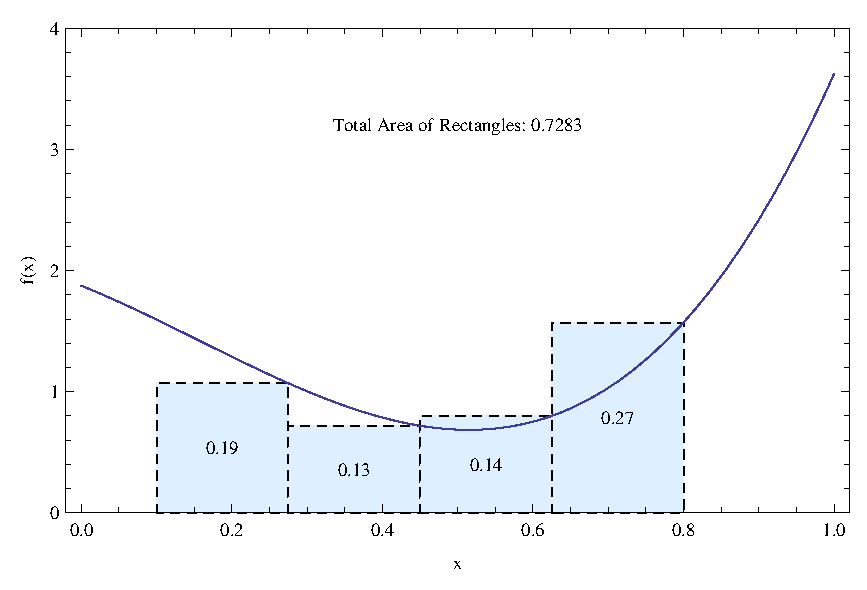
\includegraphics[scale=.6]{fig/rightrectangle-4.eps}}
\subcaptionbox{$N=6$}{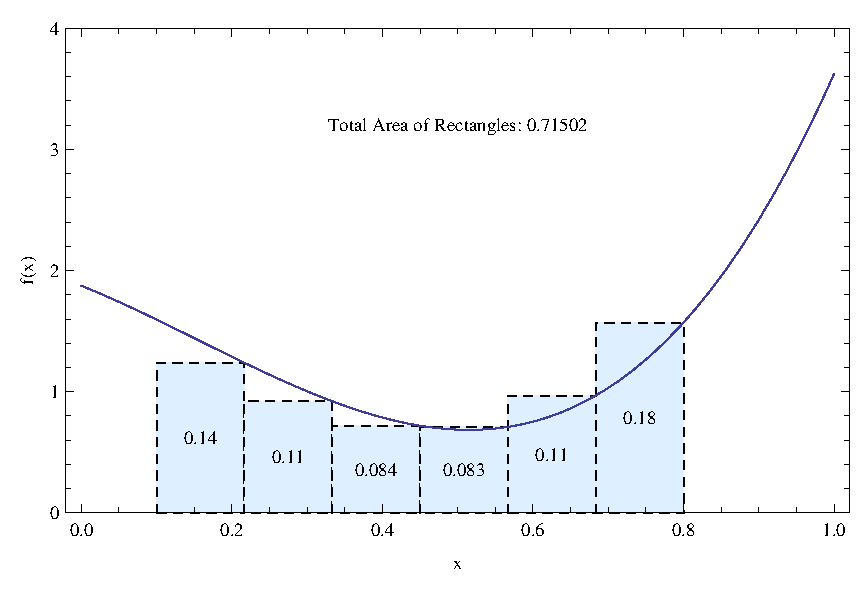
\includegraphics[scale=.6]{fig/rightrectangle-6.eps}}
\subcaptionbox{$N=10$}{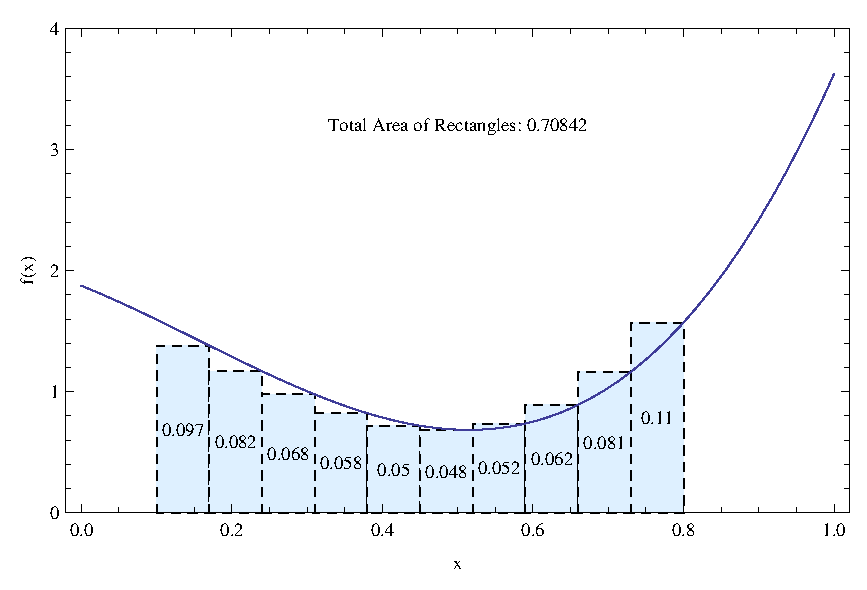
\includegraphics[scale=.6]{fig/rightrectangle-10.eps}}
\caption{Numerical integration of $f(x) = (2 x-0.5)^3+(1.5 x-1)^2-x+1$ for $x$ in $[0.1,0.8]$
by the (right) rectangle method for increasing values of $N$. The number inside each rectangle is
the area of that rectangle, and the total area is displayed on each graph.
The exact value of the integral is 0.70525.}\label{fig:rectangle}
\end{figure}

If $f(x)$ is increasing or decreasing on the interval $[a,b]$, the maximum error $E$ 
for left or right rectangular numerical integration is given by
\begin{equation}
E \leq \frac{b-a}{N}\left|f(b)-f(a)\right| \label{eq:lr-rectangle-max-error}
\end{equation}

We can create a helper function to compute the maximum error for left and right rectangle
methods using \ref{eq:lr-rectangle-max-error}. The calculated value will be used
in tests for the left and right rectangle methods to check that the result is within 
the maximum error expected for a given $a$, $b$, and $N$. 
\begin{enumspec}
\item\spec{1} Helper function \lstinline{leftRightRectangleMaxErr} returns the
maximum error expected for left or right rectangle method numerical integration. It 
takes in a reference to a pre-defined function $f$, the bounds $a$ (real) and $b$ (real) of the 
interval for definite integration, and the number $N$ (integer) of subintervals used.
The function will be entered in \lstinline{leftRightRectangleMaxErr.chpl}.
\meetsreq{5,5.1}
\end{enumspec}

\begin{chapelhelper}{leftRightRectangleMaxErr.chpl}
\begin{chapel}
proc leftRightRectangleMaxErr(a: real, b: real, N: int, f){
  return ((b-a)/N)*abs(f(b)-f(a));
}
\end{chapel}
\end{chapelhelper}

\begin{seamlessnote}
In \lstinline{seamless} vernacular, the helper files are chunks of code that are used to support
testing that the developer wants to have outside of the tests. The most likely reason being that
the code contains setup or auxiliary functions that are used for multiple tests. In our example
above, we are using some foresight and envisioning that the \lstinline{leftRightRectangleMaxErr}
function will also be used in a test for the left rectangle numerical integration function. To 
extract the helper files from your latex source files, run the following command in the same
directory as your latex source:
\begin{verbatim}
[./tutorial/] $ make helpers
\end{verbatim}
This command runs the \lstinline{helpers} target in the Makefile at the root of the 
tutorial directory (\lstinline{./tutorial/Makefile}. A Makefile is a text 
file written in a certain prescribed syntax. Together with the \lstinline{make} utility, it 
helps automate repetitive commandline tasks such as building software from its source files. 
In this case, the \lstinline{helpers} target cleans out the \lstinline{./tutorial/helper} directory and
executes the \lstinline{./util/extract\_helpers} python script with the appropriate arguments.
\end{seamlessnote}

One of the functions that we need to test our methods against is $f(x) = x^3$, 
with $a=0$, $b=1$, and $N=100$.
Since the function is increasing on the interval $[0,1]$, we can use 
the helper function that we just created to compute the maximum expected error. We are
ready to create our first test for a function that we will write to compute the definite
integral using the left rectangle method. This function will be called 
\lstinline{leftRectangleIntegration}
and will be written to \lstinline{leftRectangleIntegration.chpl}.
Since we know we have four tests to construct (Requirements \ref{req5.1} through \ref{req5.4}),
we will label the specification for this first test \ref{spec2.1}
\begin{TODO}
  Add seamless note on how to reference spec's and req's.
\end{TODO}

\begin{enumspec}
\item\spec{2.1}
Test \lstinline{leftRectangleIntegrationTest1.chpl} loads modules
\lstinline{leftRightRectangleMaxErr} and
\lstinline{leftRectangleIntegration}.
It defines a function \lstinline{f} that takes $x$ (real) and returns $x^3$ (real).
It passes $a=0.0$, $b=1.0$, $N=100$, and \lstinline{f} to the function
\lstinline{leftRightRectangleMaxErr} and stores the result in the variable
\lstinline{maximumError} (real).
It passes $a=0.0$, $b=1.0$, $N=100$, and \lstinline{f} to the function
\lstinline{leftRectangleIntegration} and stores the result in the variable
\lstinline{calculated}.
Variable \lstinline{exact: real} is initialized with the exact value of the integral from
Mathematica, 0.25.
It then checks to see if the absolute value of the difference between \lstinline{calculated} 
and \lstinline{exact} is less than or equal to \lstinline{maximumError} and sets 
\lstinline{verified: bool}. The test writes out \lstinline{verified} and a passing
test results in \lstinline{true}.
\meetsreq{5.1}
\end{enumspec}

\begin{chapelexample}{leftRectangleIntegrationTest1.chpl}
A test for \lstinline{leftRectangleIntegration}.
\begin{chapelpre}
\end{chapelpre}
\begin{chapel}
use leftRightRectangleMaxErr;
use leftRectangleIntegration;
proc f(x:real):real {
  return x**3;
} 
  
var calculated:real;
var exact:real = 0.25;  // from Mathematica
var maximumError:real = leftRightRectangleMaxErr(a = 0.0, b = 1.0, N = 100, f = f);
var verified:bool;

calculated = leftRectangleIntegration(a = 0.0, b = 1.0, N = 100, f = f);
verified = (abs(calculated - exact) <= maximumError);
writeln(verified);
\end{chapel}
\begin{chapelpost}
\end{chapelpost}
\begin{chapeloutput}
true
\end{chapeloutput}
\end{chapelexample}

\begin{seamlessnote}
Now that we have our first test, we need to extract it from the latex source and verify
that it does not pass.
To extract the test from the latex source and run it:
\begin{verbatim}
[./tutorial/] $ make tests
[./tutorial/] $ make test
\end{verbatim}
These commands run the \lstinline{tests} and \lstinline{test} targets in the same Makefile referenced above.
In this case, the \lstinline{tests} target cleans out the \lstinline{./tutorial/test} directory and
executes the \lstinline{./util/extract_tests} python script with the appropriate arguments.
The \lstinline{test} target changes to the \lstinline{./tutorial/test} directory and 
executes the \lstinline{start_test} csh script that comes with
the chapel distribution (in \lstinline{CHPL_HOME/util}). The script compiles and executes each of the
chapel source files in the test directory 
(\eg \lstinline{leftRectangleIntegrationTest.chpl} as in the example above) 
and compares the output with the contents of a file with a \lstinline{.good} extension
(\eg \lstinline{leftRectangleIntegrationTest.good} for the above test). 
The last few lines of output should look something like this:
\begin{verbatim}
[Test Summary - 150107.202408]
[Summary: #Successes = 0 | #Failures = 1 | #Futures = 0 | #Warnings = 0 ]
[END]
\end{verbatim}
\end{seamlessnote}

\begin{TODO}
  Update test target to run all targets necessary to run tests.
\end{TODO}

Another of the functions that we need to test our methods against is 
$f(x) = 1/x$, where $x$ is $[1,100]$, with 1,000 approximations. 
The exact result is the natural log of 100, or about 4.605170.
Since the function is decreasing on the interval $[1,100]$, we can again use 
the helper function in \lstinline{leftRightRectangleMaxErr.chpl} to compute the 
maximum expected error.  
Our second test 
for the left rectangle method is very similar to the first. 
\begin{enumspec}
\item\spec{2.2}
Test \lstinline{leftRectangleIntegrationTest2.chpl} loads modules
\lstinline{leftRightRectangleMaxErr} and
\lstinline{leftRectangleIntegration}.
It defines a function \lstinline{f} that takes \lstinline{x: real} and returns $1/x$.
It passes $a=1.0$, $b=100.0$, $N=1000$, and \lstinline{f} to the function
\lstinline{leftRightRectangleMaxErr} and stores the result in the variable
\lstinline{maximumError} (real).
It passes $a=1.0$, $b=100.0$, $N=1000$, and \lstinline{f} to the function
\lstinline{leftRectangleIntegration} and stores the result in the variable
\lstinline{calculated}.
Variable \lstinline{exact: real} is initialized with the exact value of the integral, 4.605170.
It then checks to see if the absolute value of the difference between \lstinline{calculated} 
and \lstinline{exact} is less than or equal to \lstinline{maximumError} and sets 
\lstinline{verified: bool}. The test writes out \lstinline{verified} and a passing
test results in \lstinline{true}.
\meetsreq{5.2}
\end{enumspec}

\begin{chapelexample}{leftRectangleIntegrationTest2.chpl}
  A test for \lstinline{leftRectangleIntegration} using $f(x) = 1/x$.
\begin{chapelpre}
\end{chapelpre}
\begin{chapel}
use leftRightRectangleMaxErr;
use leftRectangleIntegration;
proc f(x:real):real {
  return 1/x;
} 
  
var calculated:real;
var exact:real = 4.605170; 
var maximumError:real = leftRightRectangleMaxErr(a = 1.0, b = 100.0, N = 1000, f = f);
var verified:bool;

calculated = leftRectangleIntegration(a = 1.0, b = 100.0, N = 1000, f = f);
verified = (abs(calculated - exact) <= maximumError);
writeln(verified);
\end{chapel}
\begin{chapelpost}
\end{chapelpost}
\begin{chapeloutput}
true
\end{chapeloutput}
\end{chapelexample}

The code that provides the \lstinline{leftRectangleIntegration} function is straightforward.
\begin{enumspec}
\item\spec{3} Function \lstinline{leftRectangleIntegration}, for an interval
  of integration, $[a,b]$,
  takes the left end value of the interval, \lstinline{a: real}, the right end value
  of the interval, \lstinline{b: real}, the number of subintervals for the numerical
  integration, \lstinline{N: int}, and the function to be integrated, \lstinline{f}.
  The function stores the width of the subinterval calculated from Equation 
  \ref{eq:subinterval-width} in the variable \lstinline{h: real}. It initializes the variable
  \lstinline{sum: real} to zero, and for each value of $n$ in the summation of Equation~\ref{eq:rectangle},
  it computes \lstinline{x_n: real} according to the expression in Table~\ref{tab:xn-rectangle} and adds
  the value of \lstinline{f(x_n)} to \lstinline{sum: real}. The function returns the product of 
  \lstinline{sum: real} and the subinterval width, \lstinline{h: real}.
  \meetsreq{1}
\end{enumspec}

\begin{chapelsource}{leftRectangleIntegration.chpl}
\begin{chapel}
proc leftRectangleIntegration(a: real(64), b: real(64), N: int(64), f): real(64){
  var h: real(64) = (b - a)/N; 
  var sum: real(64) = 0.0;
  var x_n: real(64);
  for n in 0..N-1 {
    x_n = a + n * h;
    sum = sum + f(x_n);
  }
  return h * sum;
}
\end{chapel}
\end{chapelsource}

\begin{seamlessnote}
  We can now verify that test \lstinline{leftRectangleIntegrationTest.chpl} passes. First
  we need to extract the chapel source from our latex file and then run the test that was
  written previously:
\begin{verbatim}
[./tutorial/] $ make sources
[./tutorial/] $ make test
\end{verbatim}
These commands run the \lstinline{sources} and \lstinline{test} targets in our Makefile.
In this case, the \lstinline{sources} target cleans out the \lstinline{./tutorial/source} directory and
executes the \lstinline{./util/extract_sources} python script with the appropriate arguments, putting
the source code that we've defined in our latex file into the \lstinline{./tutorial/source} directory.
\end{seamlessnote}

\begin{TODO}
  Describe refactoring of the above code.
\end{TODO}

For a function $f$ which is twice differentiable, the maximum error $E$ is given by
the following equation:
\begin{equation}
E \leq \frac{(b-a)h^2}{24} f''(\xi) \label{eq:rectangle-max-error}
\end{equation}
for some $\xi$ in $[a,b]$.

Create a helper function to compute the maximum error:
\begin{chapelhelper}{midpointRectangularIntegrationMaximumError.chpl}
\begin{chapel}
proc midpointRectangularIntegrationMaximumError(a: real, b: real, N: int, fppxi){
  var h:real = (b-a)/N;
  return ((b-a)*h**2/24) * fppxi;
}
\end{chapel}
\end{chapelhelper}

\cleardoublepage
\sekshun{Trapezoid Integration}
\label{Trapezoid_Integration}
\index{trapezoid integration}
\index{integration!trapezoid}

The trapezoid method computes an approximation to a 
definite integral by finding the area of a collection of trapezoids whose heights are determined 
by the values of the function.  Specifically, the interval $[a,b]$ over which the function is to 
be integrated is divided into $N$ equal subintervals of length $h = (b-a)/N$. The trapezoids are 
drawn with the base along the $x$-axis.  Both the left and right corner of the side opposite the 
base lies on the graph of the function. The approximation to the integral is 
then calculated by adding up the areas of the trapezoids (base multiplied by sum of two sides 
divided by two) of the $N$ trapezoids, giving the formula:
\begin{equation}
  \int_a^b f(x) dx \approx \frac{h}{2} \left[ f(a) + 2\sum_{n=1}^{N-1} f(x_n) + f(b) \right] \label{eq:trapezoid}
\end{equation}
where 
\begin{equation}\label{eq:xn-trapezoid}
x_n = a + nh
\end{equation}
and $h$ is still given by Equation~\ref{eq:subinterval-width}.

For a function $f$ which is twice differentiable, the maximum error $E$ for the
trapezoid method is given by the following equation:
\begin{equation}
  E \leq \frac{(b-a)^3}{12 N^2} f''(\xi) \label{eq:trapezoid-max-error}
\end{equation}
for some $\xi$ in $[a,b]$.

We can use the maximum value of the second derivative 
computed in Section~\ref{sec:midpoint-rectangle-method} 
in Equation~\ref{eq:trapezoid-max-error}. 
As with the midpoint rectangle method, the trapezoid method is expected to give a very 
accurate answer for $f(x) = x$,
so we will use a value of 0.00001 for the maximum expected error for the two final tests.
The calculated maximum expected error for the tests specified in Requirements~\ref{req@5.1} and
\ref{req@5.2} are given in Table~\ref{tab:trapezoid-error}.

\begin{table}[htbp]
  \centering
  \caption{Values for expressions in Equation~\ref{eq:trapezoid-max-error} and the maximum 
    expected error of the trapezoid method of numerical integration for $f(x) = \{x^3, 1/x\}$.}
  \label{tab:trapezoid-error}
  \begin{tabular}{ccccc}
    \textbf{Function} & \textbf{Interval} & \textbf{N} & \textbf{Maximum $f''(x)$} & $E$  \\ \toprule
    $x^3$ & $[0,1]$   & 100  & 6 & 0.00005 \\ \midrule
    $1/x$ & $[1,100]$ & 1000 & 3 & 0.24257 \\ \bottomrule
  \end{tabular}
\end{table}

\begin{chapelexample}{trapezoidIntegrationTest.chpl}
  A test for \lstinline{trapezoidIntegration} using $f(x) = \{x^3, 1/x, x\}$.
  \begin{chapelpre}
  \end{chapelpre}
  \begin{chapel}
    use trapezoidIntegration;
    use testFunctions;

    var exact:real;
    var calculated:real;
    var maxErr:real;

    exact = 0.25;
    maxErr = 0.00005;
    calculated = trapezoidIntegration(a = 0.0, b = 1.0, N = 100, f = f1);
    writeln((abs(calculated - exact) <= maxErr));

    exact = 4.605170;
    maxErr = 0.24257;
    calculated = trapezoidIntegration(a = 1.0, b = 100.0, N = 1000, f = f2);
    writeln((abs(calculated - exact) <= maxErr));

    exact = 12500000;
    maxErr = 0.00001;
    calculated = trapezoidIntegration(a = 0.0, b = 5000.0, N = 5000000, f = f3);
    writeln((abs(calculated - exact) <= maxErr));

    exact = 18000000;
    maxErr = 0.00001;
    calculated = trapezoidIntegration(a = 0.0, b = 6000.0, N = 6000000, f = f3);
    writeln((abs(calculated - exact) <= maxErr));
  \end{chapel}
  \begin{chapelpost}
  \end{chapelpost}
  \begin{chapeloutput}
true
true
true
true
  \end{chapeloutput}
\end{chapelexample}

\begin{chapelsource}{trapezoidIntegration.chpl}
  \begin{chapel}
    proc trapezoidIntegration(a: real(64), b: real(64), N: int(64), f): real{
      var h: real(64) = (b - a)/N; 
      var sum: real(64) = f(a) + f(b);
      var x_n: real(64);
      for n in 1..N-1 {
        x_n = a + n * h;
        sum = sum + 2.0 * f(x_n);
      }
      return (h/2.0) * sum;
    }
  \end{chapel}
\end{chapelsource}


\cleardoublepage
\sekshun{Simpson's Rule Integration}
\label{Simpsons_Integration}
\index{Simpson's rule integration}
\index{integration!Simpson's rule}

The Simpson's rule method approximates the function with a quadratic. The particular flavor that
we are going to use here requires that the interval $[a,b]$ is subdivided into an even number of
subintervals of width $h=(b-a)/N$. 
The general Simpson's rule is given by
\begin{equation}
  \int_a^b f(x) dx \approx \frac{h}{3} \left[ f(a) + 
  4\sum_{\substack{n=1\\n \text{odd}}}^{N-1} f(x_n) + 
  4\sum_{\substack{n=2\\n \text{even}}}^{N-2} f(x_n) + 
  f(b) \right] \label{eq:simpsons}
\end{equation}
where $x_n$ is still given by Equation~\ref{eq:xn-trapezoid} and 
$h$ is still given by Equation~\ref{eq:subinterval-width}.

For a function $f$ which has a fourth derivative, the maximum error $E$ for the
Simpson's rule method is given by the following equation:
\begin{equation}
  E \leq \frac{(b-a)^5}{180 N^4} f^{(4)}(\xi) \label{eq:simpsons-max-error}
\end{equation}
for some $\xi$ in $[a,b]$.

The expected error for the Simpson's rule method for all of the tests is expected  
to be very low, so we will use a value of 0.00001 for all of them.

\begin{chapelexample}{simpsonsIntegrationTest.chpl}
  A test for \lstinline{simpsonsIntegration} using $f(x) = \{x^3, 1/x, x\}$.
  \begin{chapelpre}
  \end{chapelpre}
  \begin{chapel}
    use simpsonsIntegration;
    use testFunctions;

    var exact:real;
    var calculated:real;
    var maxErr:real;

    exact = 0.25;
    maxErr = 0.00001;
    calculated = simpsonsIntegration(a = 0.0, b = 1.0, N = 100, f = f1);
    writeln((abs(calculated - exact) <= maxErr));

    exact = 4.605170;
    maxErr = 0.00001;
    calculated = simpsonsIntegration(a = 1.0, b = 100.0, N = 1000, f = f2);
    writeln((abs(calculated - exact) <= maxErr));

    exact = 12500000;
    maxErr = 0.00001;
    calculated = simpsonsIntegration(a = 0.0, b = 5000.0, N = 5000000, f = f3);
    writeln((abs(calculated - exact) <= maxErr));

    exact = 18000000;
    maxErr = 0.00001;
    calculated = simpsonsIntegration(a = 0.0, b = 6000.0, N = 6000000, f = f3);
    writeln((abs(calculated - exact) <= maxErr));
  \end{chapel}
  \begin{chapelpost}
  \end{chapelpost}
  \begin{chapeloutput}
true
true
true
true
  \end{chapeloutput}
\end{chapelexample}

\begin{chapelsource}{simpsonsIntegration.chpl}
  \begin{chapel}
    proc simpsonsIntegration(a: real(64), b: real(64), N: int(64), f): real{
      var h: real(64) = (b - a)/N; 
      var sum: real(64) = f(a) + f(b);
      var x_n: real(64);
      for n in 1..N-1 by 2 {
        x_n = a + n * h;
        sum = sum + 4.0 * f(x_n);
      }
      for n in 2..N-2 by 2 {
        x_n = a + n * h;
        sum = sum + 2.0 * f(x_n);
      }
      return (h/3.0) * sum;
    }
  \end{chapel}
\end{chapelsource}

\begin{chapelexample}{simpsonsIntegrationParallelTest.chpl}
  A test for \lstinline{simpsonsIntegrationParallel} using $f(x) = \{x^3, 1/x, x\}$.
  \begin{chapelpre}
  \end{chapelpre}
  \begin{chapel}
    use simpsonsIntegrationParallel;
    use testFunctions;

    var exact:real;
    var calculated:real;
    var maxErr:real;

    exact = 0.25;
    maxErr = 0.00001;
    calculated = simpsonsIntegrationParallel(a = 0.0, b = 1.0, N = 100, f = f1);
    writeln((abs(calculated - exact) <= maxErr));

    exact = 4.605170;
    maxErr = 0.00001;
    calculated = simpsonsIntegrationParallel(a = 1.0, b = 100.0, N = 1000, f = f2);
    writeln((abs(calculated - exact) <= maxErr));

    exact = 12500000;
    maxErr = 0.00001;
    calculated = simpsonsIntegrationParallel(a = 0.0, b = 5000.0, N = 5000000, f = f3);
    writeln((abs(calculated - exact) <= maxErr));

    exact = 18000000;
    maxErr = 0.00001;
    calculated = simpsonsIntegrationParallel(a = 0.0, b = 6000.0, N = 6000000, f = f3);
    writeln((abs(calculated - exact) <= maxErr));
  \end{chapel}
  \begin{chapelpost}
  \end{chapelpost}
  \begin{chapeloutput}
true
true
true
true
  \end{chapeloutput}
\end{chapelexample}

\begin{chapelsource}{simpsonsIntegrationParallel.chpl}
  \begin{chapel}
    proc simpsonsIntegrationParallel(a: real(64), b: real(64), N: int(64), f): real{
      var h: real(64) = (b - a)/N; 
      var sum1$, sum2$: sync real = 0.0;
      var x_n1$, x_n2$: sync real;
      cobegin {
        for n1 in 1..N-1 by 2 {
          x_n1$ = a + n1 * h;
          sum1$ = sum1$ + 4.0 * f(x_n1$);
        }
        for n2 in 2..N-2 by 2 {
          x_n2$ = a + n2 * h;
          sum2$ = sum2$ + 2.0 * f(x_n2$);
        }
      }
      return (h/3.0) * (f(a) + sum1$ + sum2$ + f(b));
    }
  \end{chapel}
\end{chapelsource}

\begin{TODO}
  Fix chapel\_listing.tex to handle \$ characters for sync variables.
\end{TODO}

\begin{chapelexample}{simpsonsIntegrationParallelTestWithTiming.chpl}
  A test for \lstinline{simpsonsIntegration} and \lstinline{simpsonsIntegrationParallel} 
  using $f(x) = \{x^3, 1/x, x\}$ comparing timing of the parallel and serial methods.
  \begin{chapelpre}
  \end{chapelpre}
  \begin{chapel}
    use simpsonsIntegrationParallel;
    use simpsonsIntegration;
    use testFunctions;
    use Time;

    var exact:real;
    var calculated:real;
    var maxErr:real;
    var timer, timerP:Timer;
    var timerMargin: real = 0.6;

    exact = 0.25;
    maxErr = 0.00001;
    timerP.start();
    calculated = simpsonsIntegrationParallel(a = 0.0, b = 1.0, N = 100, f = f1);
    timerP.stop();
    writeln((abs(calculated - exact) <= maxErr));
    timer.start();
    calculated = simpsonsIntegration(a = 0.0, b = 1.0, N = 100, f = f1);
    timer.stop();
    writeln((abs(calculated - exact) <= maxErr));
    writeln((timerP.elapsed() < timerMargin*timer.elapsed()));

    exact = 4.605170;
    maxErr = 0.00001;
    timerP.clear();
    timerP.start();
    calculated = simpsonsIntegrationParallel(a = 1.0, b = 100.0, N = 1000, f = f2);
    timerP.stop();
    writeln((abs(calculated - exact) <= maxErr));
    timer.clear();
    timer.start();
    calculated = simpsonsIntegration(a = 1.0, b = 100.0, N = 1000, f = f2);
    timer.stop();
    writeln((abs(calculated - exact) <= maxErr));
    writeln((timerP.elapsed() < 0.5*timer.elapsed()));

    exact = 12500000;
    maxErr = 0.00001;
    timerP.clear();
    timerP.start();
    calculated = simpsonsIntegrationParallel(a = 0.0, b = 5000.0, N = 5000000, f = f3);
    timerP.stop();
    writeln((abs(calculated - exact) <= maxErr));
    timer.clear();
    timer.start();
    calculated = simpsonsIntegration(a = 0.0, b = 5000.0, N = 5000000, f = f3);
    timer.stop();
    writeln((abs(calculated - exact) <= maxErr));
    writeln((timerP.elapsed() < timerMargin*timer.elapsed()));

    exact = 18000000;
    maxErr = 0.00001;
    timerP.clear();
    timerP.start();
    calculated = simpsonsIntegrationParallel(a = 0.0, b = 6000.0, N = 6000000, f = f3);
    timerP.stop();
    writeln((abs(calculated - exact) <= maxErr));
    timer.clear();
    timer.start();
    calculated = simpsonsIntegration(a = 0.0, b = 6000.0, N = 6000000, f = f3);
    timer.stop();
    writeln((abs(calculated - exact) <= maxErr));
    writeln((timerP.elapsed() < timerMargin*timer.elapsed()));
  \end{chapel}
  \begin{chapelpost}
  \end{chapelpost}
  \begin{chapeloutput}
true
true
true
true
true
true
true
true
true
true
true
true
  \end{chapeloutput}
\end{chapelexample}

\cleardoublepage
\appendix
\begin{table}[htbp]
\centering
\caption{Requirement traceability matrix.}
\begin{tabular}{cc}
\textbf{Requirement} & \textbf{Specification}   \\ 
\toprule
\xintFor* #1 in \requirements\do {\ref{#1}&\specswithreq{#1}\\ 
  \midrule}%
\end{tabular}
\end{table}

\cleardoublepage
\markboth{Test-Driven Development with \texttt{seamless}}{Index}
\documentclass[10pt,twoside,titlepage]{seamless}
\usepackage{amsmath}
\usepackage{amssymb}
\usepackage{color}
\usepackage{times}
%\usepackage{fullpage}
\usepackage{graphicx}
\usepackage{listings}
\usepackage{longtable}
\usepackage[nottoc]{tocbibind}
\usepackage{multirow}
\usepackage{wrapfig,booktabs}
\usepackage{subcaption}
%\usepackage{cleveref}
%%
% These are special environments for adding extra information about
% code snippets which can be later extracted and used to generate test
% codes for automated testing.
%
% During LaTeX compilation, the environments defined in this file throw
% away all text within the scope of the environment, with the
% exception of 'chapelprintoutput' which prints the output (and is
% also extracted for testing purposes).
%
% Usage:
%
% - chapelexample (REQUIRED) {f.chpl}
%   This marks the start of a test.  This environment requires a
%   single argument that is the name of the Chapel test program.  This
%   filename will appear in the spec.
%
% - chapelpre
%   Any Chapel code in this scope is put *before* the code in the
%   chapel|chapelcode scope.
%
% - chapelcode|chapel
%   This is the part of the code that is in the spec.
%
% - chapelnoprint
%   This is the part of the code that goes in the test with chapelcode
%   and chapel, but does not appear in the spec.
%   
% - chapelpost
%   Any Chapel code in this scope is put *after* the code in the
%   chapel|chapelcode scope.
%
% - chapelfuture
% - chapelcompopts
% - chapelexecopts
%   The lines in these scopes are put directly into the appropriate file.
%
% - chapeloutput|chapelprintoutput (REQUIRED)
%   These environment provide the test output (.good files).  There can be
%   multiple such environments, and the filename is specified by a LaTeX
%   style comment preceeding the contents of the output.  The
%   'chapelprintoutput' scope is also outputted in the spec itself and
%   thus may contain LaTeX formatting (see GENERAL CAVEATS below)
%   
% - chapelwideoutput
%   Provides the test output for no-local tests, if that differs from the
%   normal test output.  The content of this environment is dumped into a
%   <test>.no-local.good file, along with a copy of the content of 
%   chplprintoutput.
%

%
% GENERAL CAVEATS:
%
% - Because the chapelprintoutput environment must used LaTeX
%   formatting, the script that extracts the tests must removed any
%   LaTeX specific formatting.
%
% - Using a backslash or other special LaTeX characters may also be
%   needed (e.g., \_ or \#) in the other environments for LaTex
%   parsing purposes.  Such characters are considered fragile and may
%   lead to unexpected results.
%

%
% Gobble up the text in this new box.  The text in each environment is
% dropped on the floor during LaTeX compilation.
%
\newsavebox{\teststuff}

%
% Any additional lines needed for the code snippet to run/compile
% (before and after the chapel code segment)
%
\newenvironment{chapelpre} {\begin{lrbox}{\teststuff}
\begin{minipage}{6in}}
{\end{minipage}\end{lrbox}}

\newenvironment{chapelnoprint} {\begin{lrbox}{\teststuff}
\begin{minipage}{6in}}
{\end{minipage}\end{lrbox}}

\newenvironment{chapelpost} {\begin{lrbox}{\teststuff}
\begin{minipage}{6in}}
{\end{minipage}\end{lrbox}}


%
% .future file
%
\newenvironment{chapelfuture} {\begin{lrbox}{\teststuff}
\begin{minipage}{6in}}
{\end{minipage}\end{lrbox}}

%
% .compopts file
%
\newenvironment{chapelcompopts} {\begin{lrbox}{\teststuff}
\begin{minipage}{6in}}
{\end{minipage}\end{lrbox}}

%
% .execopts file
%
\newenvironment{chapelexecopts} {\begin{lrbox}{\teststuff}
\begin{minipage}{6in}}
{\end{minipage}\end{lrbox}}


%
% .good file
% To get more than one file, use a LaTeX style comment to name the
% .good file
%
\newenvironment{chapeloutput} {\begin{lrbox}{\teststuff}
\begin{minipage}{6in}}
{\end{minipage}\end{lrbox}}

%
% .no-local.good file
% (The naming feature mentioned above does not yet work, so this
% environment is a Q&D way to get a .no-local.good file.)
%
\newenvironment{chapelwideoutput} {\begin{lrbox}{\teststuff}
\begin{minipage}{6in}}
{\end{minipage}\end{lrbox}}

%
% .prediff file
%
\newenvironment{chapelprediff} {\begin{lrbox}{\teststuff}
\begin{minipage}{6in}}
{\end{minipage}\end{lrbox}}

%
% .good file that is printed in the text of the Spec
% To get more than one file, use a LaTeX style comment to name the
% .good file
%
%\lstnewenvironment{chapelprintoutput} 
% (See chapel_listing.tex for the implementation.)

\usepackage{seamless}
\lstdefinelanguage{chapel}
  {
    morekeywords={
      align, atomic,
      begin, bool, break, by,
      class, cobegin, coforall, complex, config, const, continue,
      delete, dmapped, do, domain,
      else, enum, extern, export,
      false, for, forall,
      if, imag, in, index, inline, inout, int, iter,
      label, lambda, let, local, locale,
      module,
      new, nil, noinit,
      on, opaque, otherwise, out,
      param, proc,
      range, real, record, reduce, ref, return,
      scan, select, serial, single, sparse, string, subdomain, sync,
      then, true, type,
      uint, union, use,
      var,
      when, where, while, with,
      yield,
      zip
    },
    sensitive=false,
    mathescape=true,
    morecomment=[l]{//},
    morecomment=[s]{/*}{*/},
    morestring=[b]",
}

\lstset{
    basicstyle=\footnotesize\ttfamily,
    keywordstyle=\bfseries,
    commentstyle=\em,
    showstringspaces=false,
    flexiblecolumns=false,
    numbers=left,
    numbersep=5pt,
    numberstyle=\tiny,
    numberblanklines=false,
    stepnumber=0,
    escapeinside={(*}{*)},
    language=chapel,
  }

%\newcommand{\chpl}[1]{\lstinline[language=chapel,basicstyle=\ttfamily,keywordstyle=\bfseries]!#1!}
\newcommand{\chpl}[1]{\lstinline[language=chapel,basicstyle=\small\ttfamily,keywordstyle=]!#1!}
\newcommand{\varname}[1]{\emph{#1}}
\newcommand{\typename}[1]{\emph{#1}}
\newcommand{\fnname}[1]{\chpl{#1}}

\lstnewenvironment{chapel}{\lstset{language=chapel,xleftmargin=2pc,stepnumber=0}}{}
\lstnewenvironment{invisible}{\lstset{language=chapel,xleftmargin=2pc,stepnumber=0,keywordstyle=\bfseries\color{white},basicstyle=\small\ttfamily\color{white}}}{}
\lstnewenvironment{chapel0}{\lstset{language=chapel,stepnumber=0}}{}

\lstnewenvironment{numberedchapel}{\lstset{language=chapel,xleftmargin=15pt,stepnumber=1}}{}

\lstnewenvironment{chapelcode}{\lstset{language=chapel,stepnumber=1}}{}

% Uses the same listing style as the {chapel} environment, but keyword
% formatting is turned off.  The argument is ignored in LaTeX
% but used to name the .good file during test extraction.
% The argument must be supplied but may be empty.
% If empty it defaults to null, which signals the test extractor to 
% autogenerate the .good file name as ``<test_name>.good''.
\lstnewenvironment{chapelprintoutput}[1]
  {\lstset{language=chapel,xleftmargin=2pc,stepnumber=0,keywordstyle=}}{}

\lstnewenvironment{commandline}{\lstset{keywordstyle=,xleftmargin=2pc}}{}

\lstnewenvironment{protohead}{\lstset{language=chapel,xleftmargin=0pc,belowskip=-10pt,stepnumber=0}}{}

\newenvironment{protobody}{\begin{description}\item[\quad\quad] }{\end{description}}


%% High section numbers require different number widths
\usepackage[titles]{tocloft}
\setlength{\cftchapnumwidth}{1.3em} % Wide enough for a chapter number.
\setlength{\cftsecnumwidth}{3.2em}  % Same as cftsubsecnumwidth:
\setlength{\cftsubsecnumwidth}{3.2em} % Wide enough for three digits and two dots.
%\setlength{\cftsubsubsecnumwidth}{5.4em}
\setlength{\cftsecindent}{1.3em}    % cftchapnumwidth
\setlength{\cftsubsecindent}{1.3em} % cftchapnumwidth
\setlength{\cftsubsubsecindent}{4.5em} % cftchapnumwidth + cftsecnumwidth

%\usepackage{ifpdf}
%\ifpdf
%\usepackage[pdftex,
            %bookmarks,
            %plainpages=false,
            %breaklinks,
            %pdftitle={Test-Driven Development with seamless},
            %pdfauthor={Paul Adamson},
            %pdfsubject={seamless package, literate programming, test-driven development}
           %]{hyperref}
%\else
%\usepackage[ps2pdf]{hyperref}
%\fi

% some custom latex convenience commands
\usepackage{xspace}
\newcommand*{\eg}{\emph{e.g.}\@\xspace}
\newcommand*{\ie}{\emph{i.e.}\@\xspace}

\makeatletter
\newcommand*{\etc}{%
  \@ifnextchar{.}%
  {etc}%
  {etc.\@\xspace}%
}
\makeatother

\newcommand{\rsec}[1]
           {\S\ref{#1}}

% courtesy: http://www.iam.ubc.ca/~newbury/tex/page-set-up.html
\newcommand{\sekshun}[1]
           {
             \chapter{#1}
             \markboth{Test-Driven Development with \texttt{seamless}}{#1}
           }

\oddsidemargin 0.0in
\evensidemargin 0.5in
\textwidth 6in
\headheight 0.2in
\topmargin 0in
\headsep 0.3in
\textheight 8.5in

\makeindex
\title{Test-Driven Development with \texttt{seamless}}

\author{Paul Adamson\\
\\
}

\date{January 1, 2015}

\setcounter{tocdepth}{3}

\begin{document}

\pagestyle{empty}
%\pagenumbering{alph}

\ifpdf
\pdfbookmark[1]{Title}{titlepage}
\fi
\maketitle

\null\vfill
\noindent
\begin{center}
\copyright Paul Adamson
\end{center}

\cleardoublepage
\include{tm}
\cleardoublepage

\pagestyle{myheadings}
\markboth{Test-Driven Development with \texttt{seamless}}{Test-Driven Development with \texttt{seamless}}
%\pagenumbering{roman}

\ifpdf
\pdfbookmark[1]{Table of Contents}{tablecontents}
\fi
\tableofcontents

\cleardoublepage

\pagestyle{myheadings}
%\pagenumbering{arabic}

\setlength{\parindent}{0in}
\setlength{\parskip}{4mm plus2mm minus1mm}

%\part{Introduction}
\sekshun{Notation}
\label{Notation}
\index{notation}

Special notations are used in this specification to denote ExotiMO Chapel code
and to denote ExotiMO syntax.

ExotiMO Chapel code is represented with a fixed-width font where keywords are
bold and comments are italicized.
\begin{example}
\begin{chapel}
for i in D do   // iterate over domain D
  writeln(i);   // output indices in D
\end{chapel}
\end{example}

ExotiMO syntax is represented with standard syntax notation in which
productions define the syntax of the package.  A production is
defined in terms of non-terminal ({\it italicized}) and terminal
(non-italicized) symbols.  The complete syntax defines all of the
non-terminal symbols in terms of one another and terminal symbols.

A definition of a non-terminal symbol is a multi-line construct.  The
first line shows the name of the non-terminal that is being defined
followed by a colon.  The next lines before an empty line define the
alternative productions to define the non-terminal.
\begin{example}
The production
\begin{syntax_donotcollect}
bool-literal:
  `true'
  `false'
\end{syntax_donotcollect}
defines \sntx{bool-literal} to be either the symbol \sntx{`true'} or
\sntx{`false'}.
\end{example}
In the event that a single line of a definition needs to break across
multiple lines of text, more indentation is used to indicate that it
is a continuation of the same alternative production.

As a short-hand for cases where there are many alternatives that
define one symbol, the first line of the definition of the
non-terminal may be followed by ``one of'' to indicate that the single
line in the production defines alternatives for each symbol.
\begin{example}
The production
\begin{syntax_donotcollect}
unary-operator: one of
  + $ $ $ $ - $ $ $ $ ~ $ $ $ $ !
\end{syntax_donotcollect}
is equivalent to
\begin{syntax_donotcollect}
unary-operator:
  +
  -
  ~
  !
\end{syntax_donotcollect}
\end{example}

As a short-hand to indicate an optional symbol in the definition of a
production, the subscript ``opt'' is suffixed to the symbol.
\begin{example}
The production
\begin{syntax_donotcollect}
formal:
  formal-tag identifier formal-type[OPT] default-expression[OPT]
\end{syntax_donotcollect}
is equivalent to
\begin{syntax_donotcollect}
formal:
  formal-tag identifier formal-type default-expression
  formal-tag identifier formal-type
  formal-tag identifier default-expression
  formal-tag identifier
\end{syntax_donotcollect}
\end{example}

\cleardoublepage
\sekshun{Organization}
\label{Organization}
\index{organization}

This book is organized as follows:

\begin{description}

\item[Chapter~\ref{Notation}] Notation, introduces the notation that is used
throughout the book.

%\item[Chapter~\ref{Acknowledgments}] Acknowledgements, offers a note of
%thanks to people and projects.

\item[Chapter~\ref{Organization}] Organization, describes the contents of
each of the parts and chapters within this document.

\item[Chapter~\ref{Development_Approach}] Development Approach, describes 
the unique test-driven development process of the \lstinline{seamless} package.

\item[Chapter~\ref{Requirements}] Requirements, explains the importance of starting
with good requirements along with example scope and functional requirements for 
the numerical integration code that we will develop in the book.

\item[Chapter~\ref{Rectangle_Integration}] Rectangle Integration, documentation, source
code, and test suite for implementation of rectangle method numerical integration 
in the Chapel language.

\end{description}

\cleardoublepage
\sekshun{Development Approach}
\label{Development_Approach}
\index{development approach}

Before we dive into developing requirements and hacking away at code, a brief description of 
the \lstinline{seamless} approach to software development, a literate programming approach to 
test-driven development, is in order.  (Well, as you will see later, the \lstinline{seamless} approach
is probably better described as a ``quasi-literate programming'' approach, but I will explain
in due course.)

\section{Test-Driven Development}
Test-driven development, or TDD, is the notion that developers will improve both the design and
accuracy of their code by \textit{writing the test} for a particular feature \textit{before writing the 
code} that implements the feature according to the specification. In other words, the TDD process 
begins with writing an automated test for code that does not yet 
exist. After a test is written for a particular feature defined in the specification, the 
programmer then writes the implementing code to get the test to pass. This process is repeated until
all features in the specification are implemented. 

The idea is that by writing tests before code, rather than after, the tests will help guide
the design in small, incremental steps. Over time, this creates a well-factored and robust
codebase that is easier to modify.

\begin{TODO}
Consider adding a story about TDD.
\end{TODO}

\subsection{The Classic TDD Process}\label{tdd-classic}

\begin{TODO} The following process is almost ver batim from Rails 4 Test Prescriptions. Need to 
cite the work and tailor to technical computing/Chapel code development.
\end{TODO}

The classic TDD process goes something like this:
\begin{enumerate}
\item Create a test. The test should be short and test for one thing in your code. The test
should run automatically.
\item Make sure the test fails. Verifying the test failure before you write code helps ensure
that the test really does what you expect.
\item Write the simplest code that could possibly make the test pass. Don't worry about good
code yet. Don't look ahead. Sometimes, write just enough code to clear the current error.
\item After the test passes, refactor to improve the code. Clean up duplication. Optimize.
Create new abstractions. Refactoring is a key part of design, so don't skip this. 
\item Run the tests again to make sure you haven't changed any behavior.
\end{enumerate}

Repeat the above cycle until your code is complete. This will, in theory, ensure that your code is
always as simple as possible and completely covered by tests. 

\subsection{TDD Aids Design}

\begin{TODO}
Describe in more detail how TDD aids design. Draw from Rails Test Prescriptions, pg 5+.
\end{TODO}

\subsection{Tests as Code Documentation}
A case can be made in some domains (e.g. web development) that automated test suites 
provide an alternate means of documenting code--that
the tests are, in essence, a detailed specification of the code's behavior. This is somewhat true in
technical computing, but full documentation of scientific and engineering software requires 
more than just brief comments and example output. Surely, documentation for a function that computes 
the electron-electron repulsion integral in a quantum chemistry code must have some description
of the type of electronic wavefunction for which the code is valid!

\section{Literate Programming}
Enter stage right...literate programming. 

A typical computer program consists of a text file 
containing program code. Strewn throughout will likely be scant plain text descriptions separated out by 
``comment delimeters'' that document various aspects of the code.
Since the actual code itself is presented in a such a way that supports the syntax, ordering, and structure 
that the programming language (and hence compiler) requires, the code comments will
be relatively disorganized and disjointed if you are reading them for documentation purposes. 
The way a code suite is organized in source is generally much different than the way thorough documentation is 
developed. The plain text nature of the comments also greatly limits their information value.

In literate programming the emphasis is reversed. Instead of writing \textit{a lot of} code that contains 
\textit{some} plain text documentation, 
the literate programmer writes \textit{thorough, well-organized, and content-rich} documentation that contains 
\textit{modular and efficient} code. 
The result is that the commentary is no longer hidden within a program surrounded by 
comment delimiters; instead, it is made the main focus. 
The ``program'' becomes primarily a document directed at humans, with the 
code interspersed within the documentation, separted out by ``code delimiters'' so that it can be extracted 
out and processed into source code by literate programming tools. The nature of literate programming is 
summarized pretty well in a quote from the online documentation for the FunnelWeb literate programming
preprocessor:

\begin{quote}
``The effect of this simple shift of emphasis can be so profound as to change one's whole approach to
programming. Under the literate programming paradigm, the central activity of programming becomes that of 
conveying meaning to other intelligent beings rather than merely convincing the computer to behave in a 
particular way. It is the difference between performing and exposing a magic trick.'' 
\begin{flushright}
-FunnelWeb Tutorial Manual\cite{funnelweb-what-is-literate-programming}
\end{flushright}
\end{quote}

\label{literate-program-requirements}
The following list of requirements can be used to define a ``literate program:''\cite{childs}
\begin{enumerate}
\item The high-level language code and the associated documentation come from the same 
set of source files.
\item The documentation and high-level language code for a given aspect of the program should be 
adjacent to each other when presented to the reader.
\item The literate program should be subdivided in a logical way.
\item The program should be presented in an order that is logical from the standpoint of documentation
rather than to conform to syntactic constraints of the underlying programming language(s).
\item The documentation should include notes on open issues and future areas for development.
\item Most importantly, the documentation should include a description of the problem and its solution. 
This should include all aids such as mathematics and graphics that enhance communication of the problem 
statement and the understanding of its challenge.
\item Cross references, indices, and different fonts for text, high-level language keywords, 
variable names, and literals should be reasonably automatic and obvious in the source and the documentation.
\item The program is written in small chunks that include the documentation, definitions, and code.
\end{enumerate}

The documentation portion may be any text that aids the understanding of the problem solved by the code 
(\eg description of the algorithm that is implemented).  The documentation is often significantly 
longer than the code itself. Ideally, the problem is described in a way that is agnostic of the language
in which the code is written.  For example, documentation for code that integrates a function $f(x)$ would
have discussion of discontinuities, various integration methods available (\eg trapezoidal, Simpson), 
domain of integration, \etc. 
In addition to basic shortfalls in documentation and testing in scientific codes, a recent 
study highlighted the widespread lack of basic context in available documentation.\cite{petre}
Literate programming solves this problem, ensuring that context is created while the program
is written.

\section{Literate Programming Approach to Test-Driven Development}
Test-driven development and literate programming are certainly compatible.  In fact, they are 
complementary and their combined use is a rare actual example of ``the whole is greater
than the sum of its parts,'' especially in the context of developing scientific code.  
In one document, we can clearly outline the problem to be solved, develop a test for the 
code that we want, and document the code that solves the problem. As this is done in an incremental
manner, the scientist develops the code that solves the right problem in an efficient and robust manner.
As will be seen below, the proccess also supports several fundamental aspects of good software
engineering.

\subsection{A Better TDD Process}\label{tdd-better}

A better TDD process begins first with a ``good'' requirement specification.
Failing to write a specification is the single biggest unnecessary risk a developer
can take in a software project, resulting in greatly diminished productivity. 
For any non-trivial project (more than a few days of coding for one programmer), 
the lack of a thorough specification will always result in more time and lower quality code.
Even for trivial examples, a short, informal specification will at least help to ensure
accuracy of the resulting code.

The specification is the high-level design of the program. 
Most importantly, it clearly defines the problem that the program will solve. 
Of almost equal importance is the specification of the
basic algorithms and outputs of the code. During development of the requirement specification,
the developer should evaluate available algorithms and consider how data produced from the 
program will be used.
Even if a spec is written solely for the benefit of a lone developer, the act of 
writing the specification---describing how the program works in 
minute detail---will force design of the program.

Once a specification is in hand, an improved TDD process (section \ref{tdd-classic}) can be 
undertaken in context of literate programming:
\begin{enumerate}
\item Document the problem and its solution.
  \begin{enumerate}
  \item Describe a small part of the problem to be solved. The description should include    
all aids such as mathematics and graphics that enhance communication of the problem 
statement and the understanding of its challenge. 
  \item Solve the problem, again using all aids at your disposal (\eg math, graphics).
  \item Include appropriate references to higher level requirement specifications.
  \end{enumerate}
\item Create a test. 
\begin{enumerate}
  \item The test should be as short as possible and test for one solution in your overall
  problem.\footnote{Note here that ``one thing in your code'' is replaced with ``one
  solution in your overall problem.'' This change emphasizes the literate programming emphasis
  on documenting the problem and solution before writing code. Writing the test is another
  form of documenting the solution.}
  \item The test should run automatically.
  \item Make sure the test fails. 
\end{enumerate}
\item Create the code.
  \begin{enumerate}
  \item Write the simplest code possible to pass the test. 
  \item After the test passes, refactor to improve the code. 
  \item Run the tests again to make sure the code still passes.
  \end{enumerate}
\end{enumerate}

Repeat the above cycle until your code is complete. In theory, the resulting code will 
have the following characteristics:
\begin{itemize}
  \item completely documented
  \item simple
  \item readable
  \item completely covered by tests
  \item robust
  \item accurate
  \item maintainable
  \item reusable
\end{itemize}

\subsection{Additional Software Engineering Considerations}

\begin{TODO}
Insert description of how above approach supports good software engineering (feedback to requirements, \etc).
\end{TODO}

\section{\texttt{seamless} Package}
The \lstinline{seamless} package aims to enable a literate programming approach to test-driven
development of Chapel code. It extends slightly functionality provided in the distribution
of the Chapel language source for extracting test code from the Chapel language specification.
The following files are provided in \lstinline{seamless}:
\begin{description}
\item[/Makefile] main project Makefile
\item[/spec] directory containing the \LaTeX\xspace source for this document, including an 
example of the \lstinline{seamless} approach to developing a numerical integration code in the Chapel language
\item[/spec/Makefile] the Makefile to build this document
\item[/spec/spec.tex] the main \LaTeX\xspace file for this document; other \LaTeX\xspace files not 
listed here are self-explanatory
\item[/spec/Numerical\_Integration.tex] the chapter of this document that contains the example of a literate
programming approach to test-driven development of chapel code
\item[/spec/chapel\_listing.tex] used by the \LaTeX\xspace \lstinline{listing} package to prettyprint Chapel code
\item[/spec/chapel\_testing.tex] defines environments for adding extra information about
test code chunks 
\item[/util/extract\_tests] Python script that extracts test code from \LaTeX\xspace source
\item[/util/extract\_sources] Python script that extracts source code from \LaTeX\xspace source 
\end{description}
\begin{TODO}
combine extract python scripts and update above list
\end{TODO}

Adapting \lstinline{spec.tex} and the associated \LaTeX\xspace files for a new software project is straightforward. 
Once you've adapted the structure of the \LaTeX\xspace package in the \lstinline{\spec} directory for your
purposes, and you've written a decent requirement specification, you're ready to begin the process described in
Section \ref{tdd-better}. 
To illustrate the process, we will solve the Rosetta Code numerical integration 
task\cite{rosetta-code-numerical-integration} in Chapel. As I go through the example, I will highlight
how to use the \lstinline{seamless} package to execute the literate programming and test-driven development
approach.

As I stated above, the \lstinline{seamless} approach is ``quasi-literate'' programming.  While the approach
that I've described meets the intent of the requirements outlined in Section 
\ref{literate-program-requirements} above, it fails to fully implement one of the two main concepts of
literate programming.\cite{knuth}
The first concept, described at length above, is that code should have good documentation with all of the
supporting mathematics and graphics necessary to convey its function.

The other main concept of literate programming is that the best order to explain the parts of a program 
is not necessarily going to be the same order that the compiler needs to process the code. 
For example, you might have

\begin{verbatim}
proc readInAtoms(filename:string) {
  var infile = open(filename, iomode.r);
  var reader = infile.reader();

  // 55 lines of error handling code

  readNuclei(reader);
  readBasis(reader);

}
\end{verbatim}

When first describing the function of the above block of code, the developer wants to focus on a description of 
opening the file 
and reading in data, not discussing the error handling just because the computer language requires it to be in 
between the open and the read. You probably prefer to discuss the main logic first, returning to the error-handling 
part at some later point in the documentation, perhaps in a section of the documentation that covers error-handling
for the entire software package.


Also, for a collaborator that is reviewing code to understand and perhaps contribute to it, having all of that
error handling present in the first encounter with the code block is very distracting. It is an impediment to 
understanding the main purpose of the code.

\begin{TODO}
Reword next paragraph and describe how the seamless approach deals with it (presenting evolutions of the
code and only using the latest one).
\end{TODO}
Knuth's idea goes right to the heart of the problem. When you program in a literate programming system, you get to write the code in any order you want to. The literate programming system comes with a utility program, usually called 
\lstinline{tangle}, which permutes the code into the right order so that you can compile or execute it.
Perl doesn't have anything like tangle. You can write comments and typeset them with your favorite typesetting system, but you still have to explain the code in an order that makes sense for the perl interpreter, and not for the person who's trying to understand it.


\cleardoublepage
%\part{Requirements Specification}
\sekshun{Requirements}
\label{Requirements}
\index{requirements}

\begin{seamlessnote}
  As described in Section~\ref{tdd-better}, we must begin with good requirements. In the example shown below,
  we begin with a scope that is a brief description of the software package, summarizing the code's high-level
  capabilities. The functional requirements then spell out the specific requirements in sufficient detail that 
  every line of code can be traced back to a labeled item (\eg \textbf{R1.1}). The convention used below is that
  similar requirements are nested together, and only the most deeply nested items are numbered in a given
  chain of parent/child nestings. Each labeled item inherits the language of all of its higher level parents.
  For example, in the requirements list
  \begin{description}
    \item The code shall take inputs \chpl{a} and \chpl{b}
      \begin{description}
        \item and \chpl{c}
          \begin{description}
            \item[\textbf{R1.1}] and compute \chpl{a + b - c}
            \item[\textbf{R1.2}] and compute \chpl{a - b + c}
          \end{description}
        \item[\textbf{R2}] and compute \chpl{a * b}
      \end{description}
  \end{description}
  the Requirement~\textbf{R1.1} is "the code shall take inputs \chpl{a} and \chpl{b} and \chpl{c}
  and compute \chpl{a + b - c}; however, the Requirement~\textbf{R2} is "the code shall take 
  inputs \chpl{a} and \chpl{b} and compute \chpl{a * b}.

  To place a requirement label, use the command \lstinline!\req{x}!, where \texttt{x} is the desired 
  number (\eg \lstinline!\req{1.1}!).
\end{seamlessnote}


\section{Scope}
\label{Scope}
\index{scope}

The scope of this application is the numerical integration of arbitrary functions 
to solve the Rosetta Code numerical integration task\cite{rosetta-code-numerical-integration}
in Chapel. Solving the task requires development of functions to calculate the definite 
integral of a function ($f(x)$) using rectangular (left, right, and midpoint), trapezium, and Simpson's methods.

\section{Functional Requirements}
\label{Functional_Requirements}
\index{functional requirements}

\begin{description}
  \item The code shall have functions to calculate the definite integral of a function ($f(x)$).
  \item Available methods of integration shall include:
  \begin{description}
    \item[\req{1.1}] left rectangular
      \item[\req{1.2}] right rectangular
        \item[\req{1.3}] midpoint rectangular
    \item[\req{1.4}] trapezoid
    \item[\req{1.5}] Simpson's 
  \end{description}
  \item[\req{2}] The integration functions shall take in the upper and lower bounds ($a$ and $b$) and the number of 
approximations to make in that range ($N$). 
  \item[\req{3}] The integration functions shall return the value for the integral.
  \item The test suite shall demonstrate the code's capability by showing the results for the following cases:
  \begin{description}
    \item[\req{4.1}]
    $f(x) = x^3$, where $x$ is $[0,1]$, with 100 approximations. The exact result is 1/4, or 0.25.
    \item[\req{4.2}]
    $f(x) = 1/x$, where $x$ is $[1,100]$, with 1,000 approximations. The exact result is the natural log of 100, or about 4.605170.
    \item[\req{4.3}]
    $f(x) = x$, where $x$ is $[0,5000]$, with 5,000,000 approximations. The exact result is 12,500,000.
    \item[\req{4.4}]
    $f(x) = x$, where $x$ is $[0,6000]$, with 6,000,000 approximations. The exact result is 18,000,000.
  \end{description}
\end{description}

\cleardoublepage
%\part{Technical Specification}
\sekshun{Rectangle Integration}
\label{Rectangle_Integration}
\index{rectangle integration}
\index{integration!rectangle}

The rectangle method computes an approximation to a 
definite integral by finding the area of a collection of rectangles whose heights are determined 
by the values of the function.  Specifically, the interval $[a,b]$ over which the function is to 
be integrated is divided into $N$ equal subintervals of length $h = (b-a)/N$. The rectangles are 
drawn with one base along the $x$-axis. Depending on whether the method is left, right, or midpoint,
the left corner, right corner, or midpoint, respectively, of the side opposite the base lies on the 
graph of the function. The approximation to the integral is 
then calculated by adding up the areas (base multiplied by height) of the $N$ rectangles, 
giving the formula:
\begin{equation}
\int_a^b f(x) dx \approx h \sum_{n=0}^{N-1} f(x_n) \label{eq:rectangle}
\end{equation}
where
\begin{equation}
  h=(b-a)/N  \label{eq:subinterval-width}
\end{equation}

The formula for $x_n$ for the left, right, and midpoint methods are given in Table \ref{tab:xn-rectangle}.
As $N$ gets larger, the rectangle method becomes more accurate. This is illustrated in the series of plots
in Figure \ref{fig:rectangle}.

\begin{table}[htbp]
\centering
\caption{Formula for $x_n$ in Equation \ref{eq:rectangle} of 
rectangle numerical integration methods.} 
\label{tab:xn-rectangle}
\begin{tabular}{cc}
\textbf{Method} & \textbf{$x_n$} \\ \toprule
left & $a+nh$ \\ \midrule
right & $a+(n+1)h$ \\ \midrule
midpoint & $a+\left(n + \frac{1}{2}\right)h$ \\ \bottomrule
\end{tabular}
\end{table}

\begin{figure}
\centering
\subcaptionbox{$N=4$}{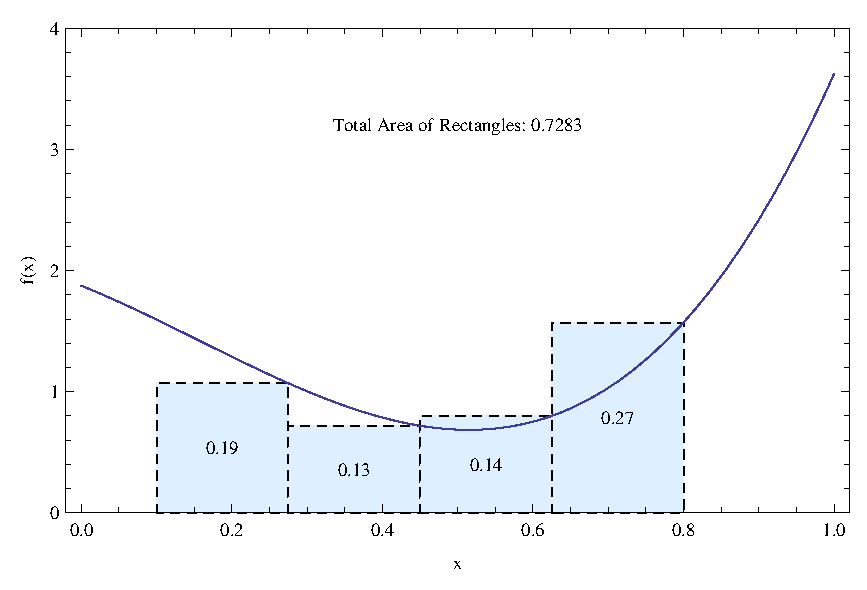
\includegraphics[scale=.6]{fig/rightrectangle-4.eps}}
\subcaptionbox{$N=6$}{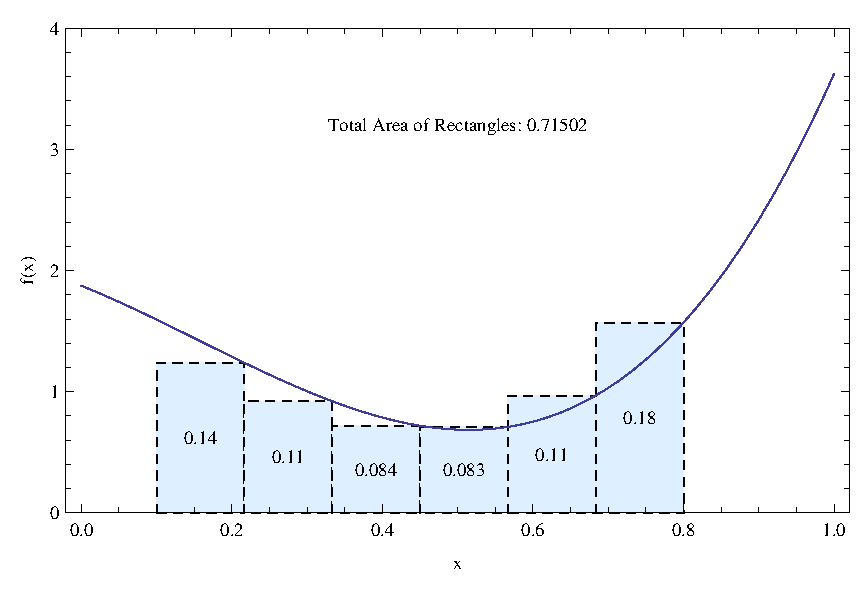
\includegraphics[scale=.6]{fig/rightrectangle-6.eps}}
\subcaptionbox{$N=10$}{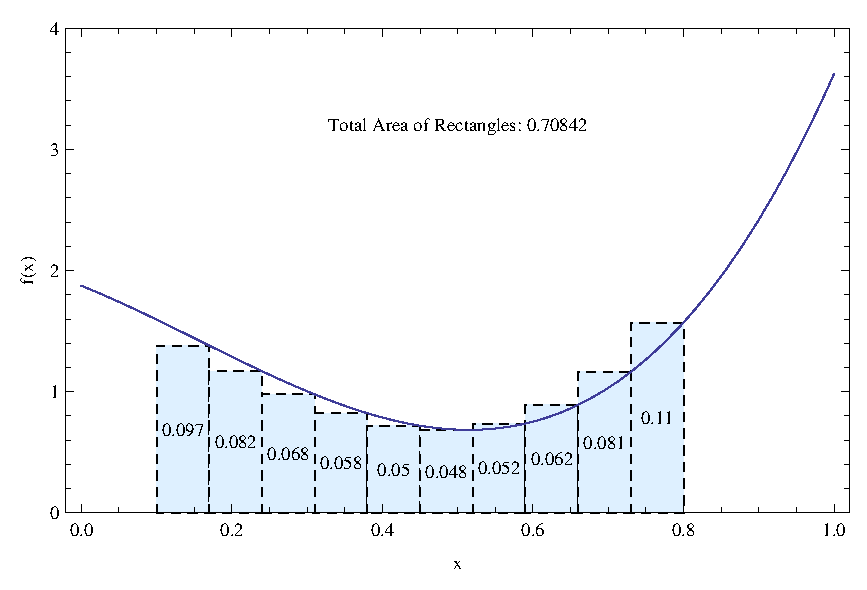
\includegraphics[scale=.6]{fig/rightrectangle-10.eps}}
\caption{Numerical integration of $f(x) = (2 x-0.5)^3+(1.5 x-1)^2-x+1$ for $x$ in $[0.1,0.8]$
by the (right) rectangle method for increasing values of $N$. The number inside each rectangle is
the area of that rectangle, and the total area is displayed on each graph.
The exact value of the integral is 0.70525.}\label{fig:rectangle}
\end{figure}

If $f(x)$ is increasing or decreasing on the interval $[a,b]$, the maximum error $E$ 
for left or right rectangular numerical integration is given by
\begin{equation}
E \leq \frac{b-a}{N}\left|f(b)-f(a)\right| \label{eq:lr-rectangle-max-error}
\end{equation}

We can create a helper function to compute the maximum error for left and right rectangle
methods using \ref{eq:lr-rectangle-max-error}. The calculated value will be used
in tests for the left and right rectangle methods to check that the result is within 
the maximum error expected for a given $a$, $b$, and $N$. 
\begin{enumspec}
\item\spec{1} Helper function \lstinline{leftRightRectangleMaxErr} returns the
maximum error expected for left or right rectangle method numerical integration. It 
takes in a reference to a pre-defined function $f$, the bounds $a$ (real) and $b$ (real) of the 
interval for definite integration, and the number $N$ (integer) of subintervals used.
The function will be entered in \lstinline{leftRightRectangleMaxErr.chpl}.
\meetsreq{5,5.1}
\end{enumspec}

\begin{chapelhelper}{leftRightRectangleMaxErr.chpl}
\begin{chapel}
proc leftRightRectangleMaxErr(a: real, b: real, N: int, f){
  return ((b-a)/N)*abs(f(b)-f(a));
}
\end{chapel}
\end{chapelhelper}

\begin{seamlessnote}
In \lstinline{seamless} vernacular, the helper files are chunks of code that are used to support
testing that the developer wants to have outside of the tests. The most likely reason being that
the code contains setup or auxiliary functions that are used for multiple tests. In our example
above, we are using some foresight and envisioning that the \lstinline{leftRightRectangleMaxErr}
function will also be used in a test for the left rectangle numerical integration function. To 
extract the helper files from your latex source files, run the following command in the same
directory as your latex source:
\begin{verbatim}
[./tutorial/] $ make helpers
\end{verbatim}
This command runs the \lstinline{helpers} target in the Makefile at the root of the 
tutorial directory (\lstinline{./tutorial/Makefile}. A Makefile is a text 
file written in a certain prescribed syntax. Together with the \lstinline{make} utility, it 
helps automate repetitive commandline tasks such as building software from its source files. 
In this case, the \lstinline{helpers} target cleans out the \lstinline{./tutorial/helper} directory and
executes the \lstinline{./util/extract\_helpers} python script with the appropriate arguments.
\end{seamlessnote}

One of the functions that we need to test our methods against is $f(x) = x^3$, 
with $a=0$, $b=1$, and $N=100$.
Since the function is increasing on the interval $[0,1]$, we can use 
the helper function that we just created to compute the maximum expected error. We are
ready to create our first test for a function that we will write to compute the definite
integral using the left rectangle method. This function will be called 
\lstinline{leftRectangleIntegration}
and will be written to \lstinline{leftRectangleIntegration.chpl}.
Since we know we have four tests to construct (Requirements \ref{req5.1} through \ref{req5.4}),
we will label the specification for this first test \ref{spec2.1}
\begin{TODO}
  Add seamless note on how to reference spec's and req's.
\end{TODO}

\begin{enumspec}
\item\spec{2.1}
Test \lstinline{leftRectangleIntegrationTest1.chpl} loads modules
\lstinline{leftRightRectangleMaxErr} and
\lstinline{leftRectangleIntegration}.
It defines a function \lstinline{f} that takes $x$ (real) and returns $x^3$ (real).
It passes $a=0.0$, $b=1.0$, $N=100$, and \lstinline{f} to the function
\lstinline{leftRightRectangleMaxErr} and stores the result in the variable
\lstinline{maximumError} (real).
It passes $a=0.0$, $b=1.0$, $N=100$, and \lstinline{f} to the function
\lstinline{leftRectangleIntegration} and stores the result in the variable
\lstinline{calculated}.
Variable \lstinline{exact: real} is initialized with the exact value of the integral from
Mathematica, 0.25.
It then checks to see if the absolute value of the difference between \lstinline{calculated} 
and \lstinline{exact} is less than or equal to \lstinline{maximumError} and sets 
\lstinline{verified: bool}. The test writes out \lstinline{verified} and a passing
test results in \lstinline{true}.
\meetsreq{5.1}
\end{enumspec}

\begin{chapelexample}{leftRectangleIntegrationTest1.chpl}
A test for \lstinline{leftRectangleIntegration}.
\begin{chapelpre}
\end{chapelpre}
\begin{chapel}
use leftRightRectangleMaxErr;
use leftRectangleIntegration;
proc f(x:real):real {
  return x**3;
} 
  
var calculated:real;
var exact:real = 0.25;  // from Mathematica
var maximumError:real = leftRightRectangleMaxErr(a = 0.0, b = 1.0, N = 100, f = f);
var verified:bool;

calculated = leftRectangleIntegration(a = 0.0, b = 1.0, N = 100, f = f);
verified = (abs(calculated - exact) <= maximumError);
writeln(verified);
\end{chapel}
\begin{chapelpost}
\end{chapelpost}
\begin{chapeloutput}
true
\end{chapeloutput}
\end{chapelexample}

\begin{seamlessnote}
Now that we have our first test, we need to extract it from the latex source and verify
that it does not pass.
To extract the test from the latex source and run it:
\begin{verbatim}
[./tutorial/] $ make tests
[./tutorial/] $ make test
\end{verbatim}
These commands run the \lstinline{tests} and \lstinline{test} targets in the same Makefile referenced above.
In this case, the \lstinline{tests} target cleans out the \lstinline{./tutorial/test} directory and
executes the \lstinline{./util/extract_tests} python script with the appropriate arguments.
The \lstinline{test} target changes to the \lstinline{./tutorial/test} directory and 
executes the \lstinline{start_test} csh script that comes with
the chapel distribution (in \lstinline{CHPL_HOME/util}). The script compiles and executes each of the
chapel source files in the test directory 
(\eg \lstinline{leftRectangleIntegrationTest.chpl} as in the example above) 
and compares the output with the contents of a file with a \lstinline{.good} extension
(\eg \lstinline{leftRectangleIntegrationTest.good} for the above test). 
The last few lines of output should look something like this:
\begin{verbatim}
[Test Summary - 150107.202408]
[Summary: #Successes = 0 | #Failures = 1 | #Futures = 0 | #Warnings = 0 ]
[END]
\end{verbatim}
\end{seamlessnote}

\begin{TODO}
  Update test target to run all targets necessary to run tests.
\end{TODO}

Another of the functions that we need to test our methods against is 
$f(x) = 1/x$, where $x$ is $[1,100]$, with 1,000 approximations. 
The exact result is the natural log of 100, or about 4.605170.
Since the function is decreasing on the interval $[1,100]$, we can again use 
the helper function in \lstinline{leftRightRectangleMaxErr.chpl} to compute the 
maximum expected error.  
Our second test 
for the left rectangle method is very similar to the first. 
\begin{enumspec}
\item\spec{2.2}
Test \lstinline{leftRectangleIntegrationTest2.chpl} loads modules
\lstinline{leftRightRectangleMaxErr} and
\lstinline{leftRectangleIntegration}.
It defines a function \lstinline{f} that takes \lstinline{x: real} and returns $1/x$.
It passes $a=1.0$, $b=100.0$, $N=1000$, and \lstinline{f} to the function
\lstinline{leftRightRectangleMaxErr} and stores the result in the variable
\lstinline{maximumError} (real).
It passes $a=1.0$, $b=100.0$, $N=1000$, and \lstinline{f} to the function
\lstinline{leftRectangleIntegration} and stores the result in the variable
\lstinline{calculated}.
Variable \lstinline{exact: real} is initialized with the exact value of the integral, 4.605170.
It then checks to see if the absolute value of the difference between \lstinline{calculated} 
and \lstinline{exact} is less than or equal to \lstinline{maximumError} and sets 
\lstinline{verified: bool}. The test writes out \lstinline{verified} and a passing
test results in \lstinline{true}.
\meetsreq{5.2}
\end{enumspec}

\begin{chapelexample}{leftRectangleIntegrationTest2.chpl}
  A test for \lstinline{leftRectangleIntegration} using $f(x) = 1/x$.
\begin{chapelpre}
\end{chapelpre}
\begin{chapel}
use leftRightRectangleMaxErr;
use leftRectangleIntegration;
proc f(x:real):real {
  return 1/x;
} 
  
var calculated:real;
var exact:real = 4.605170; 
var maximumError:real = leftRightRectangleMaxErr(a = 1.0, b = 100.0, N = 1000, f = f);
var verified:bool;

calculated = leftRectangleIntegration(a = 1.0, b = 100.0, N = 1000, f = f);
verified = (abs(calculated - exact) <= maximumError);
writeln(verified);
\end{chapel}
\begin{chapelpost}
\end{chapelpost}
\begin{chapeloutput}
true
\end{chapeloutput}
\end{chapelexample}

The code that provides the \lstinline{leftRectangleIntegration} function is straightforward.
\begin{enumspec}
\item\spec{3} Function \lstinline{leftRectangleIntegration}, for an interval
  of integration, $[a,b]$,
  takes the left end value of the interval, \lstinline{a: real}, the right end value
  of the interval, \lstinline{b: real}, the number of subintervals for the numerical
  integration, \lstinline{N: int}, and the function to be integrated, \lstinline{f}.
  The function stores the width of the subinterval calculated from Equation 
  \ref{eq:subinterval-width} in the variable \lstinline{h: real}. It initializes the variable
  \lstinline{sum: real} to zero, and for each value of $n$ in the summation of Equation~\ref{eq:rectangle},
  it computes \lstinline{x_n: real} according to the expression in Table~\ref{tab:xn-rectangle} and adds
  the value of \lstinline{f(x_n)} to \lstinline{sum: real}. The function returns the product of 
  \lstinline{sum: real} and the subinterval width, \lstinline{h: real}.
  \meetsreq{1}
\end{enumspec}

\begin{chapelsource}{leftRectangleIntegration.chpl}
\begin{chapel}
proc leftRectangleIntegration(a: real(64), b: real(64), N: int(64), f): real(64){
  var h: real(64) = (b - a)/N; 
  var sum: real(64) = 0.0;
  var x_n: real(64);
  for n in 0..N-1 {
    x_n = a + n * h;
    sum = sum + f(x_n);
  }
  return h * sum;
}
\end{chapel}
\end{chapelsource}

\begin{seamlessnote}
  We can now verify that test \lstinline{leftRectangleIntegrationTest.chpl} passes. First
  we need to extract the chapel source from our latex file and then run the test that was
  written previously:
\begin{verbatim}
[./tutorial/] $ make sources
[./tutorial/] $ make test
\end{verbatim}
These commands run the \lstinline{sources} and \lstinline{test} targets in our Makefile.
In this case, the \lstinline{sources} target cleans out the \lstinline{./tutorial/source} directory and
executes the \lstinline{./util/extract_sources} python script with the appropriate arguments, putting
the source code that we've defined in our latex file into the \lstinline{./tutorial/source} directory.
\end{seamlessnote}

\begin{TODO}
  Describe refactoring of the above code.
\end{TODO}

For a function $f$ which is twice differentiable, the maximum error $E$ is given by
the following equation:
\begin{equation}
E \leq \frac{(b-a)h^2}{24} f''(\xi) \label{eq:rectangle-max-error}
\end{equation}
for some $\xi$ in $[a,b]$.

Create a helper function to compute the maximum error:
\begin{chapelhelper}{midpointRectangularIntegrationMaximumError.chpl}
\begin{chapel}
proc midpointRectangularIntegrationMaximumError(a: real, b: real, N: int, fppxi){
  var h:real = (b-a)/N;
  return ((b-a)*h**2/24) * fppxi;
}
\end{chapel}
\end{chapelhelper}

\cleardoublepage
\appendix
\begin{table}[htbp]
\centering
\caption{Requirement traceability matrix.}
\begin{tabular}{cc}
\textbf{Requirement} & \textbf{Specification}   \\ 
\toprule
\xintFor* #1 in \requirements\do {\ref{#1}&\specswithreq{#1}\\ 
  \midrule}%
\end{tabular}
\end{table}

\cleardoublepage
\markboth{Test-Driven Development with \texttt{seamless}}{Index}
\documentclass[10pt,twoside,titlepage]{seamless}
\usepackage{amsmath}
\usepackage{amssymb}
\usepackage{color}
\usepackage{times}
%\usepackage{fullpage}
\usepackage{graphicx}
\usepackage{listings}
\usepackage{longtable}
\usepackage[nottoc]{tocbibind}
\usepackage{multirow}
\usepackage{wrapfig,booktabs}
\usepackage{subcaption}
%\usepackage{cleveref}
%%
% These are special environments for adding extra information about
% code snippets which can be later extracted and used to generate test
% codes for automated testing.
%
% During LaTeX compilation, the environments defined in this file throw
% away all text within the scope of the environment, with the
% exception of 'chapelprintoutput' which prints the output (and is
% also extracted for testing purposes).
%
% Usage:
%
% - chapelexample (REQUIRED) {f.chpl}
%   This marks the start of a test.  This environment requires a
%   single argument that is the name of the Chapel test program.  This
%   filename will appear in the spec.
%
% - chapelpre
%   Any Chapel code in this scope is put *before* the code in the
%   chapel|chapelcode scope.
%
% - chapelcode|chapel
%   This is the part of the code that is in the spec.
%
% - chapelnoprint
%   This is the part of the code that goes in the test with chapelcode
%   and chapel, but does not appear in the spec.
%   
% - chapelpost
%   Any Chapel code in this scope is put *after* the code in the
%   chapel|chapelcode scope.
%
% - chapelfuture
% - chapelcompopts
% - chapelexecopts
%   The lines in these scopes are put directly into the appropriate file.
%
% - chapeloutput|chapelprintoutput (REQUIRED)
%   These environment provide the test output (.good files).  There can be
%   multiple such environments, and the filename is specified by a LaTeX
%   style comment preceeding the contents of the output.  The
%   'chapelprintoutput' scope is also outputted in the spec itself and
%   thus may contain LaTeX formatting (see GENERAL CAVEATS below)
%   
% - chapelwideoutput
%   Provides the test output for no-local tests, if that differs from the
%   normal test output.  The content of this environment is dumped into a
%   <test>.no-local.good file, along with a copy of the content of 
%   chplprintoutput.
%

%
% GENERAL CAVEATS:
%
% - Because the chapelprintoutput environment must used LaTeX
%   formatting, the script that extracts the tests must removed any
%   LaTeX specific formatting.
%
% - Using a backslash or other special LaTeX characters may also be
%   needed (e.g., \_ or \#) in the other environments for LaTex
%   parsing purposes.  Such characters are considered fragile and may
%   lead to unexpected results.
%

%
% Gobble up the text in this new box.  The text in each environment is
% dropped on the floor during LaTeX compilation.
%
\newsavebox{\teststuff}

%
% Any additional lines needed for the code snippet to run/compile
% (before and after the chapel code segment)
%
\newenvironment{chapelpre} {\begin{lrbox}{\teststuff}
\begin{minipage}{6in}}
{\end{minipage}\end{lrbox}}

\newenvironment{chapelnoprint} {\begin{lrbox}{\teststuff}
\begin{minipage}{6in}}
{\end{minipage}\end{lrbox}}

\newenvironment{chapelpost} {\begin{lrbox}{\teststuff}
\begin{minipage}{6in}}
{\end{minipage}\end{lrbox}}


%
% .future file
%
\newenvironment{chapelfuture} {\begin{lrbox}{\teststuff}
\begin{minipage}{6in}}
{\end{minipage}\end{lrbox}}

%
% .compopts file
%
\newenvironment{chapelcompopts} {\begin{lrbox}{\teststuff}
\begin{minipage}{6in}}
{\end{minipage}\end{lrbox}}

%
% .execopts file
%
\newenvironment{chapelexecopts} {\begin{lrbox}{\teststuff}
\begin{minipage}{6in}}
{\end{minipage}\end{lrbox}}


%
% .good file
% To get more than one file, use a LaTeX style comment to name the
% .good file
%
\newenvironment{chapeloutput} {\begin{lrbox}{\teststuff}
\begin{minipage}{6in}}
{\end{minipage}\end{lrbox}}

%
% .no-local.good file
% (The naming feature mentioned above does not yet work, so this
% environment is a Q&D way to get a .no-local.good file.)
%
\newenvironment{chapelwideoutput} {\begin{lrbox}{\teststuff}
\begin{minipage}{6in}}
{\end{minipage}\end{lrbox}}

%
% .prediff file
%
\newenvironment{chapelprediff} {\begin{lrbox}{\teststuff}
\begin{minipage}{6in}}
{\end{minipage}\end{lrbox}}

%
% .good file that is printed in the text of the Spec
% To get more than one file, use a LaTeX style comment to name the
% .good file
%
%\lstnewenvironment{chapelprintoutput} 
% (See chapel_listing.tex for the implementation.)

\usepackage{seamless}
\lstdefinelanguage{chapel}
  {
    morekeywords={
      align, atomic,
      begin, bool, break, by,
      class, cobegin, coforall, complex, config, const, continue,
      delete, dmapped, do, domain,
      else, enum, extern, export,
      false, for, forall,
      if, imag, in, index, inline, inout, int, iter,
      label, lambda, let, local, locale,
      module,
      new, nil, noinit,
      on, opaque, otherwise, out,
      param, proc,
      range, real, record, reduce, ref, return,
      scan, select, serial, single, sparse, string, subdomain, sync,
      then, true, type,
      uint, union, use,
      var,
      when, where, while, with,
      yield,
      zip
    },
    sensitive=false,
    mathescape=true,
    morecomment=[l]{//},
    morecomment=[s]{/*}{*/},
    morestring=[b]",
}

\lstset{
    basicstyle=\footnotesize\ttfamily,
    keywordstyle=\bfseries,
    commentstyle=\em,
    showstringspaces=false,
    flexiblecolumns=false,
    numbers=left,
    numbersep=5pt,
    numberstyle=\tiny,
    numberblanklines=false,
    stepnumber=0,
    escapeinside={(*}{*)},
    language=chapel,
  }

%\newcommand{\chpl}[1]{\lstinline[language=chapel,basicstyle=\ttfamily,keywordstyle=\bfseries]!#1!}
\newcommand{\chpl}[1]{\lstinline[language=chapel,basicstyle=\small\ttfamily,keywordstyle=]!#1!}
\newcommand{\varname}[1]{\emph{#1}}
\newcommand{\typename}[1]{\emph{#1}}
\newcommand{\fnname}[1]{\chpl{#1}}

\lstnewenvironment{chapel}{\lstset{language=chapel,xleftmargin=2pc,stepnumber=0}}{}
\lstnewenvironment{invisible}{\lstset{language=chapel,xleftmargin=2pc,stepnumber=0,keywordstyle=\bfseries\color{white},basicstyle=\small\ttfamily\color{white}}}{}
\lstnewenvironment{chapel0}{\lstset{language=chapel,stepnumber=0}}{}

\lstnewenvironment{numberedchapel}{\lstset{language=chapel,xleftmargin=15pt,stepnumber=1}}{}

\lstnewenvironment{chapelcode}{\lstset{language=chapel,stepnumber=1}}{}

% Uses the same listing style as the {chapel} environment, but keyword
% formatting is turned off.  The argument is ignored in LaTeX
% but used to name the .good file during test extraction.
% The argument must be supplied but may be empty.
% If empty it defaults to null, which signals the test extractor to 
% autogenerate the .good file name as ``<test_name>.good''.
\lstnewenvironment{chapelprintoutput}[1]
  {\lstset{language=chapel,xleftmargin=2pc,stepnumber=0,keywordstyle=}}{}

\lstnewenvironment{commandline}{\lstset{keywordstyle=,xleftmargin=2pc}}{}

\lstnewenvironment{protohead}{\lstset{language=chapel,xleftmargin=0pc,belowskip=-10pt,stepnumber=0}}{}

\newenvironment{protobody}{\begin{description}\item[\quad\quad] }{\end{description}}


%% High section numbers require different number widths
\usepackage[titles]{tocloft}
\setlength{\cftchapnumwidth}{1.3em} % Wide enough for a chapter number.
\setlength{\cftsecnumwidth}{3.2em}  % Same as cftsubsecnumwidth:
\setlength{\cftsubsecnumwidth}{3.2em} % Wide enough for three digits and two dots.
%\setlength{\cftsubsubsecnumwidth}{5.4em}
\setlength{\cftsecindent}{1.3em}    % cftchapnumwidth
\setlength{\cftsubsecindent}{1.3em} % cftchapnumwidth
\setlength{\cftsubsubsecindent}{4.5em} % cftchapnumwidth + cftsecnumwidth

%\usepackage{ifpdf}
%\ifpdf
%\usepackage[pdftex,
            %bookmarks,
            %plainpages=false,
            %breaklinks,
            %pdftitle={Test-Driven Development with seamless},
            %pdfauthor={Paul Adamson},
            %pdfsubject={seamless package, literate programming, test-driven development}
           %]{hyperref}
%\else
%\usepackage[ps2pdf]{hyperref}
%\fi

% some custom latex convenience commands
\usepackage{xspace}
\newcommand*{\eg}{\emph{e.g.}\@\xspace}
\newcommand*{\ie}{\emph{i.e.}\@\xspace}

\makeatletter
\newcommand*{\etc}{%
  \@ifnextchar{.}%
  {etc}%
  {etc.\@\xspace}%
}
\makeatother

\newcommand{\rsec}[1]
           {\S\ref{#1}}

% courtesy: http://www.iam.ubc.ca/~newbury/tex/page-set-up.html
\newcommand{\sekshun}[1]
           {
             \chapter{#1}
             \markboth{Test-Driven Development with \texttt{seamless}}{#1}
           }

\oddsidemargin 0.0in
\evensidemargin 0.5in
\textwidth 6in
\headheight 0.2in
\topmargin 0in
\headsep 0.3in
\textheight 8.5in

\makeindex
\title{Test-Driven Development with \texttt{seamless}}

\author{Paul Adamson\\
\\
}

\date{January 1, 2015}

\setcounter{tocdepth}{3}

\begin{document}

\pagestyle{empty}
%\pagenumbering{alph}

\ifpdf
\pdfbookmark[1]{Title}{titlepage}
\fi
\maketitle

\null\vfill
\noindent
\begin{center}
\copyright Paul Adamson
\end{center}

\cleardoublepage
\include{tm}
\cleardoublepage

\pagestyle{myheadings}
\markboth{Test-Driven Development with \texttt{seamless}}{Test-Driven Development with \texttt{seamless}}
%\pagenumbering{roman}

\ifpdf
\pdfbookmark[1]{Table of Contents}{tablecontents}
\fi
\tableofcontents

\cleardoublepage

\pagestyle{myheadings}
%\pagenumbering{arabic}

\setlength{\parindent}{0in}
\setlength{\parskip}{4mm plus2mm minus1mm}

%\part{Introduction}
\sekshun{Notation}
\label{Notation}
\index{notation}

Special notations are used in this specification to denote ExotiMO Chapel code
and to denote ExotiMO syntax.

ExotiMO Chapel code is represented with a fixed-width font where keywords are
bold and comments are italicized.
\begin{example}
\begin{chapel}
for i in D do   // iterate over domain D
  writeln(i);   // output indices in D
\end{chapel}
\end{example}

ExotiMO syntax is represented with standard syntax notation in which
productions define the syntax of the package.  A production is
defined in terms of non-terminal ({\it italicized}) and terminal
(non-italicized) symbols.  The complete syntax defines all of the
non-terminal symbols in terms of one another and terminal symbols.

A definition of a non-terminal symbol is a multi-line construct.  The
first line shows the name of the non-terminal that is being defined
followed by a colon.  The next lines before an empty line define the
alternative productions to define the non-terminal.
\begin{example}
The production
\begin{syntax_donotcollect}
bool-literal:
  `true'
  `false'
\end{syntax_donotcollect}
defines \sntx{bool-literal} to be either the symbol \sntx{`true'} or
\sntx{`false'}.
\end{example}
In the event that a single line of a definition needs to break across
multiple lines of text, more indentation is used to indicate that it
is a continuation of the same alternative production.

As a short-hand for cases where there are many alternatives that
define one symbol, the first line of the definition of the
non-terminal may be followed by ``one of'' to indicate that the single
line in the production defines alternatives for each symbol.
\begin{example}
The production
\begin{syntax_donotcollect}
unary-operator: one of
  + $ $ $ $ - $ $ $ $ ~ $ $ $ $ !
\end{syntax_donotcollect}
is equivalent to
\begin{syntax_donotcollect}
unary-operator:
  +
  -
  ~
  !
\end{syntax_donotcollect}
\end{example}

As a short-hand to indicate an optional symbol in the definition of a
production, the subscript ``opt'' is suffixed to the symbol.
\begin{example}
The production
\begin{syntax_donotcollect}
formal:
  formal-tag identifier formal-type[OPT] default-expression[OPT]
\end{syntax_donotcollect}
is equivalent to
\begin{syntax_donotcollect}
formal:
  formal-tag identifier formal-type default-expression
  formal-tag identifier formal-type
  formal-tag identifier default-expression
  formal-tag identifier
\end{syntax_donotcollect}
\end{example}

\cleardoublepage
\sekshun{Organization}
\label{Organization}
\index{organization}

This book is organized as follows:

\begin{description}

\item[Chapter~\ref{Notation}] Notation, introduces the notation that is used
throughout the book.

%\item[Chapter~\ref{Acknowledgments}] Acknowledgements, offers a note of
%thanks to people and projects.

\item[Chapter~\ref{Organization}] Organization, describes the contents of
each of the parts and chapters within this document.

\item[Chapter~\ref{Development_Approach}] Development Approach, describes 
the unique test-driven development process of the \lstinline{seamless} package.

\item[Chapter~\ref{Requirements}] Requirements, explains the importance of starting
with good requirements along with example scope and functional requirements for 
the numerical integration code that we will develop in the book.

\item[Chapter~\ref{Rectangle_Integration}] Rectangle Integration, documentation, source
code, and test suite for implementation of rectangle method numerical integration 
in the Chapel language.

\end{description}

\cleardoublepage
\sekshun{Development Approach}
\label{Development_Approach}
\index{development approach}

Before we dive into developing requirements and hacking away at code, a brief description of 
the \lstinline{seamless} approach to software development, a literate programming approach to 
test-driven development, is in order.  (Well, as you will see later, the \lstinline{seamless} approach
is probably better described as a ``quasi-literate programming'' approach, but I will explain
in due course.)

\section{Test-Driven Development}
Test-driven development, or TDD, is the notion that developers will improve both the design and
accuracy of their code by \textit{writing the test} for a particular feature \textit{before writing the 
code} that implements the feature according to the specification. In other words, the TDD process 
begins with writing an automated test for code that does not yet 
exist. After a test is written for a particular feature defined in the specification, the 
programmer then writes the implementing code to get the test to pass. This process is repeated until
all features in the specification are implemented. 

The idea is that by writing tests before code, rather than after, the tests will help guide
the design in small, incremental steps. Over time, this creates a well-factored and robust
codebase that is easier to modify.

\begin{TODO}
Consider adding a story about TDD.
\end{TODO}

\subsection{The Classic TDD Process}\label{tdd-classic}

\begin{TODO} The following process is almost ver batim from Rails 4 Test Prescriptions. Need to 
cite the work and tailor to technical computing/Chapel code development.
\end{TODO}

The classic TDD process goes something like this:
\begin{enumerate}
\item Create a test. The test should be short and test for one thing in your code. The test
should run automatically.
\item Make sure the test fails. Verifying the test failure before you write code helps ensure
that the test really does what you expect.
\item Write the simplest code that could possibly make the test pass. Don't worry about good
code yet. Don't look ahead. Sometimes, write just enough code to clear the current error.
\item After the test passes, refactor to improve the code. Clean up duplication. Optimize.
Create new abstractions. Refactoring is a key part of design, so don't skip this. 
\item Run the tests again to make sure you haven't changed any behavior.
\end{enumerate}

Repeat the above cycle until your code is complete. This will, in theory, ensure that your code is
always as simple as possible and completely covered by tests. 

\subsection{TDD Aids Design}

\begin{TODO}
Describe in more detail how TDD aids design. Draw from Rails Test Prescriptions, pg 5+.
\end{TODO}

\subsection{Tests as Code Documentation}
A case can be made in some domains (e.g. web development) that automated test suites 
provide an alternate means of documenting code--that
the tests are, in essence, a detailed specification of the code's behavior. This is somewhat true in
technical computing, but full documentation of scientific and engineering software requires 
more than just brief comments and example output. Surely, documentation for a function that computes 
the electron-electron repulsion integral in a quantum chemistry code must have some description
of the type of electronic wavefunction for which the code is valid!

\section{Literate Programming}
Enter stage right...literate programming. 

A typical computer program consists of a text file 
containing program code. Strewn throughout will likely be scant plain text descriptions separated out by 
``comment delimeters'' that document various aspects of the code.
Since the actual code itself is presented in a such a way that supports the syntax, ordering, and structure 
that the programming language (and hence compiler) requires, the code comments will
be relatively disorganized and disjointed if you are reading them for documentation purposes. 
The way a code suite is organized in source is generally much different than the way thorough documentation is 
developed. The plain text nature of the comments also greatly limits their information value.

In literate programming the emphasis is reversed. Instead of writing \textit{a lot of} code that contains 
\textit{some} plain text documentation, 
the literate programmer writes \textit{thorough, well-organized, and content-rich} documentation that contains 
\textit{modular and efficient} code. 
The result is that the commentary is no longer hidden within a program surrounded by 
comment delimiters; instead, it is made the main focus. 
The ``program'' becomes primarily a document directed at humans, with the 
code interspersed within the documentation, separted out by ``code delimiters'' so that it can be extracted 
out and processed into source code by literate programming tools. The nature of literate programming is 
summarized pretty well in a quote from the online documentation for the FunnelWeb literate programming
preprocessor:

\begin{quote}
``The effect of this simple shift of emphasis can be so profound as to change one's whole approach to
programming. Under the literate programming paradigm, the central activity of programming becomes that of 
conveying meaning to other intelligent beings rather than merely convincing the computer to behave in a 
particular way. It is the difference between performing and exposing a magic trick.'' 
\begin{flushright}
-FunnelWeb Tutorial Manual\cite{funnelweb-what-is-literate-programming}
\end{flushright}
\end{quote}

\label{literate-program-requirements}
The following list of requirements can be used to define a ``literate program:''\cite{childs}
\begin{enumerate}
\item The high-level language code and the associated documentation come from the same 
set of source files.
\item The documentation and high-level language code for a given aspect of the program should be 
adjacent to each other when presented to the reader.
\item The literate program should be subdivided in a logical way.
\item The program should be presented in an order that is logical from the standpoint of documentation
rather than to conform to syntactic constraints of the underlying programming language(s).
\item The documentation should include notes on open issues and future areas for development.
\item Most importantly, the documentation should include a description of the problem and its solution. 
This should include all aids such as mathematics and graphics that enhance communication of the problem 
statement and the understanding of its challenge.
\item Cross references, indices, and different fonts for text, high-level language keywords, 
variable names, and literals should be reasonably automatic and obvious in the source and the documentation.
\item The program is written in small chunks that include the documentation, definitions, and code.
\end{enumerate}

The documentation portion may be any text that aids the understanding of the problem solved by the code 
(\eg description of the algorithm that is implemented).  The documentation is often significantly 
longer than the code itself. Ideally, the problem is described in a way that is agnostic of the language
in which the code is written.  For example, documentation for code that integrates a function $f(x)$ would
have discussion of discontinuities, various integration methods available (\eg trapezoidal, Simpson), 
domain of integration, \etc. 
In addition to basic shortfalls in documentation and testing in scientific codes, a recent 
study highlighted the widespread lack of basic context in available documentation.\cite{petre}
Literate programming solves this problem, ensuring that context is created while the program
is written.

\section{Literate Programming Approach to Test-Driven Development}
Test-driven development and literate programming are certainly compatible.  In fact, they are 
complementary and their combined use is a rare actual example of ``the whole is greater
than the sum of its parts,'' especially in the context of developing scientific code.  
In one document, we can clearly outline the problem to be solved, develop a test for the 
code that we want, and document the code that solves the problem. As this is done in an incremental
manner, the scientist develops the code that solves the right problem in an efficient and robust manner.
As will be seen below, the proccess also supports several fundamental aspects of good software
engineering.

\subsection{A Better TDD Process}\label{tdd-better}

A better TDD process begins first with a ``good'' requirement specification.
Failing to write a specification is the single biggest unnecessary risk a developer
can take in a software project, resulting in greatly diminished productivity. 
For any non-trivial project (more than a few days of coding for one programmer), 
the lack of a thorough specification will always result in more time and lower quality code.
Even for trivial examples, a short, informal specification will at least help to ensure
accuracy of the resulting code.

The specification is the high-level design of the program. 
Most importantly, it clearly defines the problem that the program will solve. 
Of almost equal importance is the specification of the
basic algorithms and outputs of the code. During development of the requirement specification,
the developer should evaluate available algorithms and consider how data produced from the 
program will be used.
Even if a spec is written solely for the benefit of a lone developer, the act of 
writing the specification---describing how the program works in 
minute detail---will force design of the program.

Once a specification is in hand, an improved TDD process (section \ref{tdd-classic}) can be 
undertaken in context of literate programming:
\begin{enumerate}
\item Document the problem and its solution.
  \begin{enumerate}
  \item Describe a small part of the problem to be solved. The description should include    
all aids such as mathematics and graphics that enhance communication of the problem 
statement and the understanding of its challenge. 
  \item Solve the problem, again using all aids at your disposal (\eg math, graphics).
  \item Include appropriate references to higher level requirement specifications.
  \end{enumerate}
\item Create a test. 
\begin{enumerate}
  \item The test should be as short as possible and test for one solution in your overall
  problem.\footnote{Note here that ``one thing in your code'' is replaced with ``one
  solution in your overall problem.'' This change emphasizes the literate programming emphasis
  on documenting the problem and solution before writing code. Writing the test is another
  form of documenting the solution.}
  \item The test should run automatically.
  \item Make sure the test fails. 
\end{enumerate}
\item Create the code.
  \begin{enumerate}
  \item Write the simplest code possible to pass the test. 
  \item After the test passes, refactor to improve the code. 
  \item Run the tests again to make sure the code still passes.
  \end{enumerate}
\end{enumerate}

Repeat the above cycle until your code is complete. In theory, the resulting code will 
have the following characteristics:
\begin{itemize}
  \item completely documented
  \item simple
  \item readable
  \item completely covered by tests
  \item robust
  \item accurate
  \item maintainable
  \item reusable
\end{itemize}

\subsection{Additional Software Engineering Considerations}

\begin{TODO}
Insert description of how above approach supports good software engineering (feedback to requirements, \etc).
\end{TODO}

\section{\texttt{seamless} Package}
The \lstinline{seamless} package aims to enable a literate programming approach to test-driven
development of Chapel code. It extends slightly functionality provided in the distribution
of the Chapel language source for extracting test code from the Chapel language specification.
The following files are provided in \lstinline{seamless}:
\begin{description}
\item[/Makefile] main project Makefile
\item[/spec] directory containing the \LaTeX\xspace source for this document, including an 
example of the \lstinline{seamless} approach to developing a numerical integration code in the Chapel language
\item[/spec/Makefile] the Makefile to build this document
\item[/spec/spec.tex] the main \LaTeX\xspace file for this document; other \LaTeX\xspace files not 
listed here are self-explanatory
\item[/spec/Numerical\_Integration.tex] the chapter of this document that contains the example of a literate
programming approach to test-driven development of chapel code
\item[/spec/chapel\_listing.tex] used by the \LaTeX\xspace \lstinline{listing} package to prettyprint Chapel code
\item[/spec/chapel\_testing.tex] defines environments for adding extra information about
test code chunks 
\item[/util/extract\_tests] Python script that extracts test code from \LaTeX\xspace source
\item[/util/extract\_sources] Python script that extracts source code from \LaTeX\xspace source 
\end{description}
\begin{TODO}
combine extract python scripts and update above list
\end{TODO}

Adapting \lstinline{spec.tex} and the associated \LaTeX\xspace files for a new software project is straightforward. 
Once you've adapted the structure of the \LaTeX\xspace package in the \lstinline{\spec} directory for your
purposes, and you've written a decent requirement specification, you're ready to begin the process described in
Section \ref{tdd-better}. 
To illustrate the process, we will solve the Rosetta Code numerical integration 
task\cite{rosetta-code-numerical-integration} in Chapel. As I go through the example, I will highlight
how to use the \lstinline{seamless} package to execute the literate programming and test-driven development
approach.

As I stated above, the \lstinline{seamless} approach is ``quasi-literate'' programming.  While the approach
that I've described meets the intent of the requirements outlined in Section 
\ref{literate-program-requirements} above, it fails to fully implement one of the two main concepts of
literate programming.\cite{knuth}
The first concept, described at length above, is that code should have good documentation with all of the
supporting mathematics and graphics necessary to convey its function.

The other main concept of literate programming is that the best order to explain the parts of a program 
is not necessarily going to be the same order that the compiler needs to process the code. 
For example, you might have

\begin{verbatim}
proc readInAtoms(filename:string) {
  var infile = open(filename, iomode.r);
  var reader = infile.reader();

  // 55 lines of error handling code

  readNuclei(reader);
  readBasis(reader);

}
\end{verbatim}

When first describing the function of the above block of code, the developer wants to focus on a description of 
opening the file 
and reading in data, not discussing the error handling just because the computer language requires it to be in 
between the open and the read. You probably prefer to discuss the main logic first, returning to the error-handling 
part at some later point in the documentation, perhaps in a section of the documentation that covers error-handling
for the entire software package.


Also, for a collaborator that is reviewing code to understand and perhaps contribute to it, having all of that
error handling present in the first encounter with the code block is very distracting. It is an impediment to 
understanding the main purpose of the code.

\begin{TODO}
Reword next paragraph and describe how the seamless approach deals with it (presenting evolutions of the
code and only using the latest one).
\end{TODO}
Knuth's idea goes right to the heart of the problem. When you program in a literate programming system, you get to write the code in any order you want to. The literate programming system comes with a utility program, usually called 
\lstinline{tangle}, which permutes the code into the right order so that you can compile or execute it.
Perl doesn't have anything like tangle. You can write comments and typeset them with your favorite typesetting system, but you still have to explain the code in an order that makes sense for the perl interpreter, and not for the person who's trying to understand it.


\cleardoublepage
%\part{Requirements Specification}
\sekshun{Requirements}
\label{Requirements}
\index{requirements}

\begin{seamlessnote}
  As described in Section~\ref{tdd-better}, we must begin with good requirements. In the example shown below,
  we begin with a scope that is a brief description of the software package, summarizing the code's high-level
  capabilities. The functional requirements then spell out the specific requirements in sufficient detail that 
  every line of code can be traced back to a labeled item (\eg \textbf{R1.1}). The convention used below is that
  similar requirements are nested together, and only the most deeply nested items are numbered in a given
  chain of parent/child nestings. Each labeled item inherits the language of all of its higher level parents.
  For example, in the requirements list
  \begin{description}
    \item The code shall take inputs \chpl{a} and \chpl{b}
      \begin{description}
        \item and \chpl{c}
          \begin{description}
            \item[\textbf{R1.1}] and compute \chpl{a + b - c}
            \item[\textbf{R1.2}] and compute \chpl{a - b + c}
          \end{description}
        \item[\textbf{R2}] and compute \chpl{a * b}
      \end{description}
  \end{description}
  the Requirement~\textbf{R1.1} is "the code shall take inputs \chpl{a} and \chpl{b} and \chpl{c}
  and compute \chpl{a + b - c}; however, the Requirement~\textbf{R2} is "the code shall take 
  inputs \chpl{a} and \chpl{b} and compute \chpl{a * b}.

  To place a requirement label, use the command \lstinline!\req{x}!, where \texttt{x} is the desired 
  number (\eg \lstinline!\req{1.1}!).
\end{seamlessnote}


\section{Scope}
\label{Scope}
\index{scope}

The scope of this application is the numerical integration of arbitrary functions 
to solve the Rosetta Code numerical integration task\cite{rosetta-code-numerical-integration}
in Chapel. Solving the task requires development of functions to calculate the definite 
integral of a function ($f(x)$) using rectangular (left, right, and midpoint), trapezium, and Simpson's methods.

\section{Functional Requirements}
\label{Functional_Requirements}
\index{functional requirements}

\begin{description}
  \item The code shall have functions to calculate the definite integral of a function ($f(x)$).
  \item Available methods of integration shall include:
  \begin{description}
    \item[\req{1.1}] left rectangular
      \item[\req{1.2}] right rectangular
        \item[\req{1.3}] midpoint rectangular
    \item[\req{1.4}] trapezoid
    \item[\req{1.5}] Simpson's 
  \end{description}
  \item[\req{2}] The integration functions shall take in the upper and lower bounds ($a$ and $b$) and the number of 
approximations to make in that range ($N$). 
  \item[\req{3}] The integration functions shall return the value for the integral.
  \item The test suite shall demonstrate the code's capability by showing the results for the following cases:
  \begin{description}
    \item[\req{4.1}]
    $f(x) = x^3$, where $x$ is $[0,1]$, with 100 approximations. The exact result is 1/4, or 0.25.
    \item[\req{4.2}]
    $f(x) = 1/x$, where $x$ is $[1,100]$, with 1,000 approximations. The exact result is the natural log of 100, or about 4.605170.
    \item[\req{4.3}]
    $f(x) = x$, where $x$ is $[0,5000]$, with 5,000,000 approximations. The exact result is 12,500,000.
    \item[\req{4.4}]
    $f(x) = x$, where $x$ is $[0,6000]$, with 6,000,000 approximations. The exact result is 18,000,000.
  \end{description}
\end{description}

\cleardoublepage
%\part{Technical Specification}
\sekshun{Rectangle Integration}
\label{Rectangle_Integration}
\index{rectangle integration}
\index{integration!rectangle}

The rectangle method computes an approximation to a 
definite integral by finding the area of a collection of rectangles whose heights are determined 
by the values of the function.  Specifically, the interval $[a,b]$ over which the function is to 
be integrated is divided into $N$ equal subintervals of length $h = (b-a)/N$. The rectangles are 
drawn with one base along the $x$-axis. Depending on whether the method is left, right, or midpoint,
the left corner, right corner, or midpoint, respectively, of the side opposite the base lies on the 
graph of the function. The approximation to the integral is 
then calculated by adding up the areas (base multiplied by height) of the $N$ rectangles, 
giving the formula:
\begin{equation}
\int_a^b f(x) dx \approx h \sum_{n=0}^{N-1} f(x_n) \label{eq:rectangle}
\end{equation}
where
\begin{equation}
  h=(b-a)/N  \label{eq:subinterval-width}
\end{equation}

The formula for $x_n$ for the left, right, and midpoint methods are given in Table \ref{tab:xn-rectangle}.
As $N$ gets larger, the rectangle method becomes more accurate. This is illustrated in the series of plots
in Figure \ref{fig:rectangle}.

\begin{table}[htbp]
\centering
\caption{Formula for $x_n$ in Equation \ref{eq:rectangle} of 
rectangle numerical integration methods.} 
\label{tab:xn-rectangle}
\begin{tabular}{cc}
\textbf{Method} & \textbf{$x_n$} \\ \toprule
left & $a+nh$ \\ \midrule
right & $a+(n+1)h$ \\ \midrule
midpoint & $a+\left(n + \frac{1}{2}\right)h$ \\ \bottomrule
\end{tabular}
\end{table}

\begin{figure}
\centering
\subcaptionbox{$N=4$}{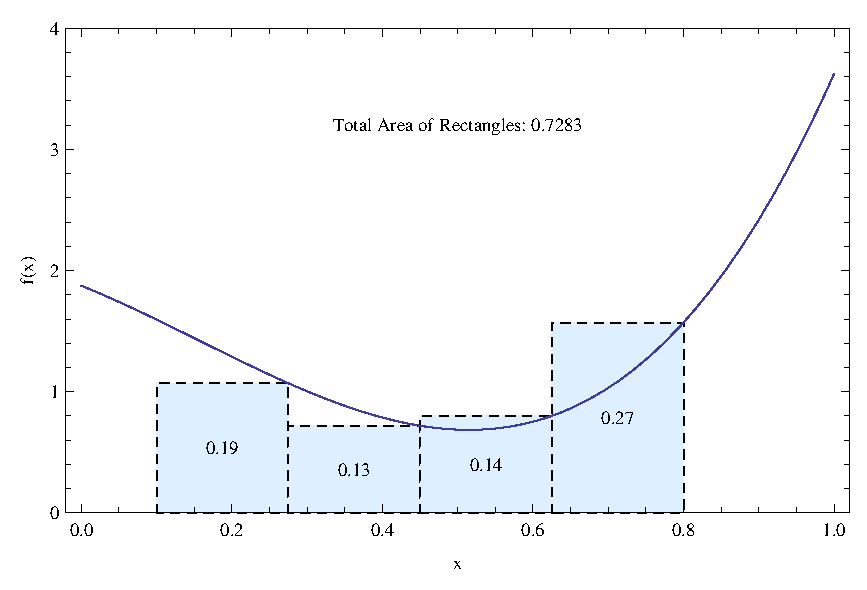
\includegraphics[scale=.6]{fig/rightrectangle-4.eps}}
\subcaptionbox{$N=6$}{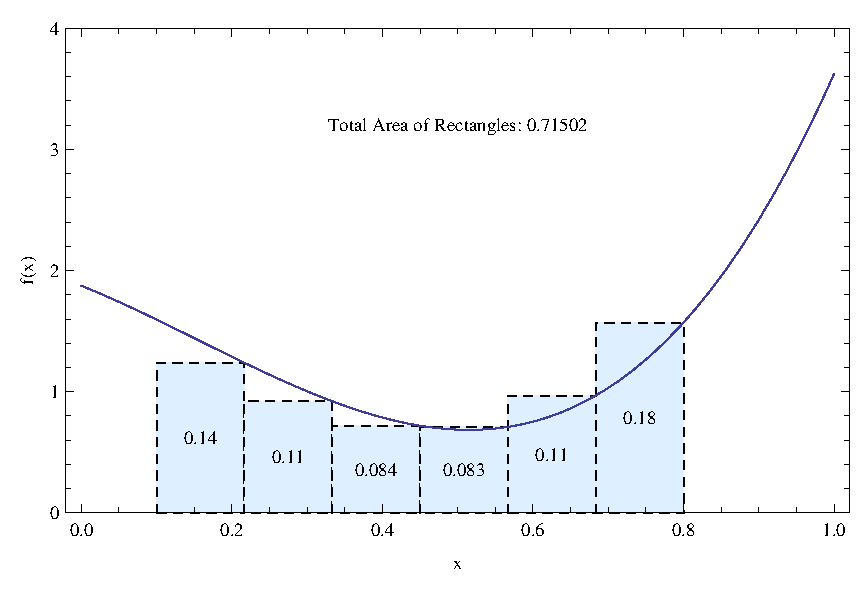
\includegraphics[scale=.6]{fig/rightrectangle-6.eps}}
\subcaptionbox{$N=10$}{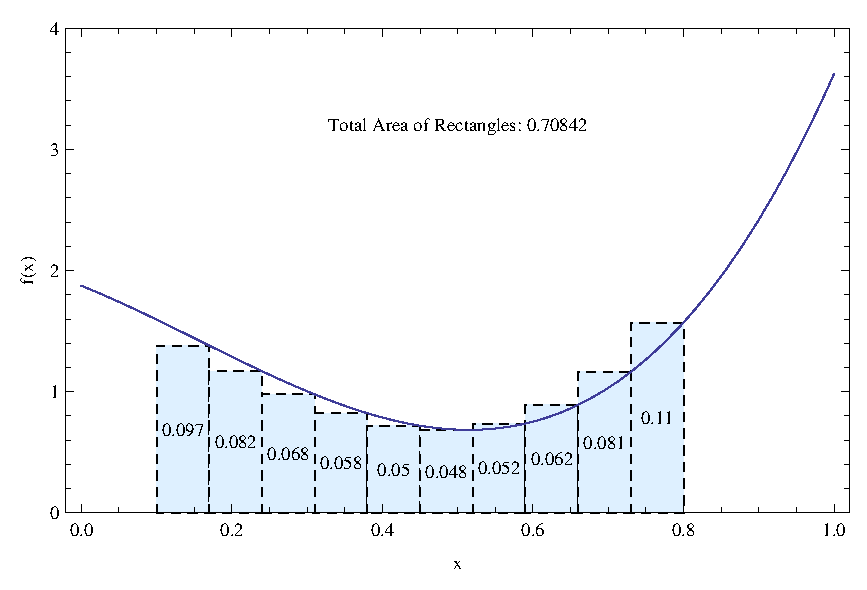
\includegraphics[scale=.6]{fig/rightrectangle-10.eps}}
\caption{Numerical integration of $f(x) = (2 x-0.5)^3+(1.5 x-1)^2-x+1$ for $x$ in $[0.1,0.8]$
by the (right) rectangle method for increasing values of $N$. The number inside each rectangle is
the area of that rectangle, and the total area is displayed on each graph.
The exact value of the integral is 0.70525.}\label{fig:rectangle}
\end{figure}

If $f(x)$ is increasing or decreasing on the interval $[a,b]$, the maximum error $E$ 
for left or right rectangular numerical integration is given by
\begin{equation}
E \leq \frac{b-a}{N}\left|f(b)-f(a)\right| \label{eq:lr-rectangle-max-error}
\end{equation}

We can create a helper function to compute the maximum error for left and right rectangle
methods using \ref{eq:lr-rectangle-max-error}. The calculated value will be used
in tests for the left and right rectangle methods to check that the result is within 
the maximum error expected for a given $a$, $b$, and $N$. 
\begin{enumspec}
\item\spec{1} Helper function \lstinline{leftRightRectangleMaxErr} returns the
maximum error expected for left or right rectangle method numerical integration. It 
takes in a reference to a pre-defined function $f$, the bounds $a$ (real) and $b$ (real) of the 
interval for definite integration, and the number $N$ (integer) of subintervals used.
The function will be entered in \lstinline{leftRightRectangleMaxErr.chpl}.
\meetsreq{5,5.1}
\end{enumspec}

\begin{chapelhelper}{leftRightRectangleMaxErr.chpl}
\begin{chapel}
proc leftRightRectangleMaxErr(a: real, b: real, N: int, f){
  return ((b-a)/N)*abs(f(b)-f(a));
}
\end{chapel}
\end{chapelhelper}

\begin{seamlessnote}
In \lstinline{seamless} vernacular, the helper files are chunks of code that are used to support
testing that the developer wants to have outside of the tests. The most likely reason being that
the code contains setup or auxiliary functions that are used for multiple tests. In our example
above, we are using some foresight and envisioning that the \lstinline{leftRightRectangleMaxErr}
function will also be used in a test for the left rectangle numerical integration function. To 
extract the helper files from your latex source files, run the following command in the same
directory as your latex source:
\begin{verbatim}
[./tutorial/] $ make helpers
\end{verbatim}
This command runs the \lstinline{helpers} target in the Makefile at the root of the 
tutorial directory (\lstinline{./tutorial/Makefile}. A Makefile is a text 
file written in a certain prescribed syntax. Together with the \lstinline{make} utility, it 
helps automate repetitive commandline tasks such as building software from its source files. 
In this case, the \lstinline{helpers} target cleans out the \lstinline{./tutorial/helper} directory and
executes the \lstinline{./util/extract\_helpers} python script with the appropriate arguments.
\end{seamlessnote}

One of the functions that we need to test our methods against is $f(x) = x^3$, 
with $a=0$, $b=1$, and $N=100$.
Since the function is increasing on the interval $[0,1]$, we can use 
the helper function that we just created to compute the maximum expected error. We are
ready to create our first test for a function that we will write to compute the definite
integral using the left rectangle method. This function will be called 
\lstinline{leftRectangleIntegration}
and will be written to \lstinline{leftRectangleIntegration.chpl}.
Since we know we have four tests to construct (Requirements \ref{req5.1} through \ref{req5.4}),
we will label the specification for this first test \ref{spec2.1}
\begin{TODO}
  Add seamless note on how to reference spec's and req's.
\end{TODO}

\begin{enumspec}
\item\spec{2.1}
Test \lstinline{leftRectangleIntegrationTest1.chpl} loads modules
\lstinline{leftRightRectangleMaxErr} and
\lstinline{leftRectangleIntegration}.
It defines a function \lstinline{f} that takes $x$ (real) and returns $x^3$ (real).
It passes $a=0.0$, $b=1.0$, $N=100$, and \lstinline{f} to the function
\lstinline{leftRightRectangleMaxErr} and stores the result in the variable
\lstinline{maximumError} (real).
It passes $a=0.0$, $b=1.0$, $N=100$, and \lstinline{f} to the function
\lstinline{leftRectangleIntegration} and stores the result in the variable
\lstinline{calculated}.
Variable \lstinline{exact: real} is initialized with the exact value of the integral from
Mathematica, 0.25.
It then checks to see if the absolute value of the difference between \lstinline{calculated} 
and \lstinline{exact} is less than or equal to \lstinline{maximumError} and sets 
\lstinline{verified: bool}. The test writes out \lstinline{verified} and a passing
test results in \lstinline{true}.
\meetsreq{5.1}
\end{enumspec}

\begin{chapelexample}{leftRectangleIntegrationTest1.chpl}
A test for \lstinline{leftRectangleIntegration}.
\begin{chapelpre}
\end{chapelpre}
\begin{chapel}
use leftRightRectangleMaxErr;
use leftRectangleIntegration;
proc f(x:real):real {
  return x**3;
} 
  
var calculated:real;
var exact:real = 0.25;  // from Mathematica
var maximumError:real = leftRightRectangleMaxErr(a = 0.0, b = 1.0, N = 100, f = f);
var verified:bool;

calculated = leftRectangleIntegration(a = 0.0, b = 1.0, N = 100, f = f);
verified = (abs(calculated - exact) <= maximumError);
writeln(verified);
\end{chapel}
\begin{chapelpost}
\end{chapelpost}
\begin{chapeloutput}
true
\end{chapeloutput}
\end{chapelexample}

\begin{seamlessnote}
Now that we have our first test, we need to extract it from the latex source and verify
that it does not pass.
To extract the test from the latex source and run it:
\begin{verbatim}
[./tutorial/] $ make tests
[./tutorial/] $ make test
\end{verbatim}
These commands run the \lstinline{tests} and \lstinline{test} targets in the same Makefile referenced above.
In this case, the \lstinline{tests} target cleans out the \lstinline{./tutorial/test} directory and
executes the \lstinline{./util/extract_tests} python script with the appropriate arguments.
The \lstinline{test} target changes to the \lstinline{./tutorial/test} directory and 
executes the \lstinline{start_test} csh script that comes with
the chapel distribution (in \lstinline{CHPL_HOME/util}). The script compiles and executes each of the
chapel source files in the test directory 
(\eg \lstinline{leftRectangleIntegrationTest.chpl} as in the example above) 
and compares the output with the contents of a file with a \lstinline{.good} extension
(\eg \lstinline{leftRectangleIntegrationTest.good} for the above test). 
The last few lines of output should look something like this:
\begin{verbatim}
[Test Summary - 150107.202408]
[Summary: #Successes = 0 | #Failures = 1 | #Futures = 0 | #Warnings = 0 ]
[END]
\end{verbatim}
\end{seamlessnote}

\begin{TODO}
  Update test target to run all targets necessary to run tests.
\end{TODO}

Another of the functions that we need to test our methods against is 
$f(x) = 1/x$, where $x$ is $[1,100]$, with 1,000 approximations. 
The exact result is the natural log of 100, or about 4.605170.
Since the function is decreasing on the interval $[1,100]$, we can again use 
the helper function in \lstinline{leftRightRectangleMaxErr.chpl} to compute the 
maximum expected error.  
Our second test 
for the left rectangle method is very similar to the first. 
\begin{enumspec}
\item\spec{2.2}
Test \lstinline{leftRectangleIntegrationTest2.chpl} loads modules
\lstinline{leftRightRectangleMaxErr} and
\lstinline{leftRectangleIntegration}.
It defines a function \lstinline{f} that takes \lstinline{x: real} and returns $1/x$.
It passes $a=1.0$, $b=100.0$, $N=1000$, and \lstinline{f} to the function
\lstinline{leftRightRectangleMaxErr} and stores the result in the variable
\lstinline{maximumError} (real).
It passes $a=1.0$, $b=100.0$, $N=1000$, and \lstinline{f} to the function
\lstinline{leftRectangleIntegration} and stores the result in the variable
\lstinline{calculated}.
Variable \lstinline{exact: real} is initialized with the exact value of the integral, 4.605170.
It then checks to see if the absolute value of the difference between \lstinline{calculated} 
and \lstinline{exact} is less than or equal to \lstinline{maximumError} and sets 
\lstinline{verified: bool}. The test writes out \lstinline{verified} and a passing
test results in \lstinline{true}.
\meetsreq{5.2}
\end{enumspec}

\begin{chapelexample}{leftRectangleIntegrationTest2.chpl}
  A test for \lstinline{leftRectangleIntegration} using $f(x) = 1/x$.
\begin{chapelpre}
\end{chapelpre}
\begin{chapel}
use leftRightRectangleMaxErr;
use leftRectangleIntegration;
proc f(x:real):real {
  return 1/x;
} 
  
var calculated:real;
var exact:real = 4.605170; 
var maximumError:real = leftRightRectangleMaxErr(a = 1.0, b = 100.0, N = 1000, f = f);
var verified:bool;

calculated = leftRectangleIntegration(a = 1.0, b = 100.0, N = 1000, f = f);
verified = (abs(calculated - exact) <= maximumError);
writeln(verified);
\end{chapel}
\begin{chapelpost}
\end{chapelpost}
\begin{chapeloutput}
true
\end{chapeloutput}
\end{chapelexample}

The code that provides the \lstinline{leftRectangleIntegration} function is straightforward.
\begin{enumspec}
\item\spec{3} Function \lstinline{leftRectangleIntegration}, for an interval
  of integration, $[a,b]$,
  takes the left end value of the interval, \lstinline{a: real}, the right end value
  of the interval, \lstinline{b: real}, the number of subintervals for the numerical
  integration, \lstinline{N: int}, and the function to be integrated, \lstinline{f}.
  The function stores the width of the subinterval calculated from Equation 
  \ref{eq:subinterval-width} in the variable \lstinline{h: real}. It initializes the variable
  \lstinline{sum: real} to zero, and for each value of $n$ in the summation of Equation~\ref{eq:rectangle},
  it computes \lstinline{x_n: real} according to the expression in Table~\ref{tab:xn-rectangle} and adds
  the value of \lstinline{f(x_n)} to \lstinline{sum: real}. The function returns the product of 
  \lstinline{sum: real} and the subinterval width, \lstinline{h: real}.
  \meetsreq{1}
\end{enumspec}

\begin{chapelsource}{leftRectangleIntegration.chpl}
\begin{chapel}
proc leftRectangleIntegration(a: real(64), b: real(64), N: int(64), f): real(64){
  var h: real(64) = (b - a)/N; 
  var sum: real(64) = 0.0;
  var x_n: real(64);
  for n in 0..N-1 {
    x_n = a + n * h;
    sum = sum + f(x_n);
  }
  return h * sum;
}
\end{chapel}
\end{chapelsource}

\begin{seamlessnote}
  We can now verify that test \lstinline{leftRectangleIntegrationTest.chpl} passes. First
  we need to extract the chapel source from our latex file and then run the test that was
  written previously:
\begin{verbatim}
[./tutorial/] $ make sources
[./tutorial/] $ make test
\end{verbatim}
These commands run the \lstinline{sources} and \lstinline{test} targets in our Makefile.
In this case, the \lstinline{sources} target cleans out the \lstinline{./tutorial/source} directory and
executes the \lstinline{./util/extract_sources} python script with the appropriate arguments, putting
the source code that we've defined in our latex file into the \lstinline{./tutorial/source} directory.
\end{seamlessnote}

\begin{TODO}
  Describe refactoring of the above code.
\end{TODO}

For a function $f$ which is twice differentiable, the maximum error $E$ is given by
the following equation:
\begin{equation}
E \leq \frac{(b-a)h^2}{24} f''(\xi) \label{eq:rectangle-max-error}
\end{equation}
for some $\xi$ in $[a,b]$.

Create a helper function to compute the maximum error:
\begin{chapelhelper}{midpointRectangularIntegrationMaximumError.chpl}
\begin{chapel}
proc midpointRectangularIntegrationMaximumError(a: real, b: real, N: int, fppxi){
  var h:real = (b-a)/N;
  return ((b-a)*h**2/24) * fppxi;
}
\end{chapel}
\end{chapelhelper}

\cleardoublepage
\appendix
\begin{table}[htbp]
\centering
\caption{Requirement traceability matrix.}
\begin{tabular}{cc}
\textbf{Requirement} & \textbf{Specification}   \\ 
\toprule
\xintFor* #1 in \requirements\do {\ref{#1}&\specswithreq{#1}\\ 
  \midrule}%
\end{tabular}
\end{table}

\cleardoublepage
\markboth{Test-Driven Development with \texttt{seamless}}{Index}
\documentclass[10pt,twoside,titlepage]{seamless}
\usepackage{amsmath}
\usepackage{amssymb}
\usepackage{color}
\usepackage{times}
%\usepackage{fullpage}
\usepackage{graphicx}
\usepackage{listings}
\usepackage{longtable}
\usepackage[nottoc]{tocbibind}
\usepackage{multirow}
\usepackage{wrapfig,booktabs}
\usepackage{subcaption}
%\usepackage{cleveref}
%\input{chapel_testing}
\usepackage{seamless}
\input{chapel_listing}

%% High section numbers require different number widths
\usepackage[titles]{tocloft}
\setlength{\cftchapnumwidth}{1.3em} % Wide enough for a chapter number.
\setlength{\cftsecnumwidth}{3.2em}  % Same as cftsubsecnumwidth:
\setlength{\cftsubsecnumwidth}{3.2em} % Wide enough for three digits and two dots.
%\setlength{\cftsubsubsecnumwidth}{5.4em}
\setlength{\cftsecindent}{1.3em}    % cftchapnumwidth
\setlength{\cftsubsecindent}{1.3em} % cftchapnumwidth
\setlength{\cftsubsubsecindent}{4.5em} % cftchapnumwidth + cftsecnumwidth

%\usepackage{ifpdf}
%\ifpdf
%\usepackage[pdftex,
            %bookmarks,
            %plainpages=false,
            %breaklinks,
            %pdftitle={Test-Driven Development with seamless},
            %pdfauthor={Paul Adamson},
            %pdfsubject={seamless package, literate programming, test-driven development}
           %]{hyperref}
%\else
%\usepackage[ps2pdf]{hyperref}
%\fi

% some custom latex convenience commands
\usepackage{xspace}
\newcommand*{\eg}{\emph{e.g.}\@\xspace}
\newcommand*{\ie}{\emph{i.e.}\@\xspace}

\makeatletter
\newcommand*{\etc}{%
  \@ifnextchar{.}%
  {etc}%
  {etc.\@\xspace}%
}
\makeatother

\newcommand{\rsec}[1]
           {\S\ref{#1}}

% courtesy: http://www.iam.ubc.ca/~newbury/tex/page-set-up.html
\newcommand{\sekshun}[1]
           {
             \chapter{#1}
             \markboth{Test-Driven Development with \texttt{seamless}}{#1}
           }

\oddsidemargin 0.0in
\evensidemargin 0.5in
\textwidth 6in
\headheight 0.2in
\topmargin 0in
\headsep 0.3in
\textheight 8.5in

\makeindex
\title{Test-Driven Development with \texttt{seamless}}

\author{Paul Adamson\\
\\
}

\date{January 1, 2015}

\setcounter{tocdepth}{3}

\begin{document}

\pagestyle{empty}
%\pagenumbering{alph}

\ifpdf
\pdfbookmark[1]{Title}{titlepage}
\fi
\maketitle

\null\vfill
\noindent
\begin{center}
\copyright Paul Adamson
\end{center}

\cleardoublepage
\include{tm}
\cleardoublepage

\pagestyle{myheadings}
\markboth{Test-Driven Development with \texttt{seamless}}{Test-Driven Development with \texttt{seamless}}
%\pagenumbering{roman}

\ifpdf
\pdfbookmark[1]{Table of Contents}{tablecontents}
\fi
\tableofcontents

\cleardoublepage

\pagestyle{myheadings}
%\pagenumbering{arabic}

\setlength{\parindent}{0in}
\setlength{\parskip}{4mm plus2mm minus1mm}

%\part{Introduction}
\input{Notation}
\cleardoublepage
\input{Organization}
\cleardoublepage
\input{Development_Approach}
\cleardoublepage
%\part{Requirements Specification}
\input{Requirements}
\cleardoublepage
%\part{Technical Specification}
\input{Rectangle_Integration}
\cleardoublepage
\appendix
\input{Requirement_Traceability}
\cleardoublepage
\markboth{Test-Driven Development with \texttt{seamless}}{Index}
\input{Numerical_Integration.ind}

\bibliographystyle{plain}       
\bibliography{master} 

\end{document}


\bibliographystyle{plain}       
\bibliography{master} 

\end{document}


\bibliographystyle{plain}       
\bibliography{master} 

\end{document}


\bibliographystyle{plain}       
\bibliography{master} 

\end{document}
